\graphicspath{{figures/chapter2/}}
\onehalfspacing

\chapter{Back to the Past: Reconstructing Glacier Topography with Archival Aerial Images
  (1977-2009)}\label{ch:2}
  
\vfill

\newthought{This chapter is based on:}

\noindent De Gaetani, C. I., Ioli, F., \& Pinto, L. (2021). Aerial and UAV Images for
Photogrammetric Analysis of Belvedere Glacier Evolution in the Period 1977–2019. Remote
Sensing, 13(18), 3787. \url{https://doi.org/10.3390/rs13183787}

\newpage

\section{Introduction}\label{sec:2:introduction}

To understand the long-term dynamics of an alpine glacier, gathering information from the past becomes mandatory. 
Geomorphological studies benefit from three-dimensional topographic representations, which accurately describe the topography surfaces and quantify their variation over time~\citep{chandler1995steady}.
Traditionally, image datasets acquired by metric cameras mounted onboard planes have been used to build maps through analytical stereo plotters and traditional photogrammetric techniques. 
Image orientation experienced improvements with the incorporation of GNSS-INS sensors for precise camera positioning and orientation
~\citep{Forlani_pinto2001, jacobsen2004issues}.

The emergence of digital photogrammetry in the late 1990s and the advent of automated methods for finding homologous points between images catalyzed a shift towards automated processing of extensive image collections. 
Since then, photogrammetry has become a widely used, cost- and time-effective approach for geoscience research~\citep{Lane2000}.
This transformation, coupled with the development of Structure-from-Motion (SfM) and Multi-View Stereo (MVS) algorithms and the availability of affordable digital cameras, has established photogrammetry as an indispensable technique for geomorphological research and glacier monitoring.

Despite millions of analog photographs documenting land surface change taken in the past century being available in historical archives, only a tiny fraction of these photographs have been digitally scanned and can be used with modern photogrammetric techniques. 
Scanned historical aerial image archives allow for \textit{going back in time} and derive accurate historical DSMs and orthophotos for long-term measurements of surface change ~\citep{Micheletti2015}.

Examples of applications of historical archive photogrammetry for documenting geomorphological processes include fluvial geomorphology~\citep{Bakker2017, lane2010quantification}, gravitational mass movement processes~\citep{chandler1995steady, walstra2007historical, schwab2008landsliding}, mapping and land cover estimation~\citep{Giordano2018} and permafrost and glacial processes~\citep{kaab2002monitoring, Kaufmann2003, keutterling2006monitoring, mondino2008multi, Fischer2011}.

Recently, several modern photogrammetric software packages, including Agisoft Metashape\footnote{\url{https://www.agisoft.com/}}, Pix4DMapper\footnote{\url{https://www.pix4d.com/product/pix4dmapper-photogrammetry-software/}}, ERDAS IMAGINE\footnote{\url{https://hexagon.com/products/imagine-photogrammetry}}, MicMac~\citep{rupnik2017micmac, Zhang2021} together with a recent sPyMicMac addition~\citep{McNabb2020} and NASA AMES Stereo Pipeline~\citep{Beyer2018}, have implemented support for processing archival images with fiducial marks defining the camera interior orientation. 
Moreover, the Swiss Federal Office of Topography SwissTopo has recently digitalized, cataloged, and published a large collection of grayscale and color historical aerial images on their website~\citep{Heisig2021}, representing a virtuosus example of promoting open data practices.
In this context, several authors employed modern photogrammetric techniques with historical archive images for reconstructing glaciers' 3D topography in the past, including glaciers in Antartica~\citep{Child2021, Dahle2024}, North America~\citep{Knuth2023} and in the Alpine region~\citep{Molg2017, poli2020use}.

This chapter aims to reconstruct the long-term evolution of the Belvedere Glacier between 1977 and 2019 by utilizing historical archival images and modern digital photogrammetry.
To this end, three archival datasets captured by analog metric cameras in 1977, 1991, and 2001 were combined with data from a more recent aerial survey (2009) and a UAV flight (2019).
These surveys are distributed across the timeline with a relatively consistent interval of approximately ten years, allowing us to track the glacier's morphological evolution and quantify volumetric changes. 

Notably, the 2001 dataset captured the 3D topography of the Belvedere Glacier during a peculiar surge-type event \citep{Haeberli2002} occurred between 2000 and 2002 (see \secref{sec:1:belvedereglacier} for more  details)
This event marked the glacier's maximum extension since the Little Ice Age, and its resulting moraines remain visible today.
Consequently, analyzing the Belvedere Glacier's long-term evolution since 1977 enables us to quantify the progression of a glacier that underwent a rapid expansion followed by a critical regression and thinning. This process continues to this day.

% swiss archive \citet{Heisig2021}
% Glaciers: 
%  - historical aerial photogrammetry \citet{kaab2002monitoring, Kaufmann2003, keutterling2006monitoring, mondino2008multi, Fischer2011}
%  - modern photogrammetry\citet{Molg2017, poli2020use, Child2021, Knuth2023, Dahle2024} 
% photogrammetry to geomorphology~\citet{chandler1995steady, walstra2007historical, schwab2008landsliding, Micheletti2015, Bakker2017}
% land cover \citet{Giordano2018}
% historical aerial images for semantic segment \citet{Dahle2024}
% swiss archive \citet{Heisig2021}
% Moreover, in the past ten years, the increasing development of unmanned aerial vehicles (UAVs), low-cost sensors, and structure-from-motion (SfM) techniques have drastically reduced the need for highly specific and expensive equipment for large-scale glacier monitoring [17]. High-spatial-resolution volume variation [18,19,20,21] and high-frequency displacement and surface velocity fields [22,23,24,25,26] can be derived even by a single research group with simplified logistics and resource allocation.


\section{Datasets}\label{sec:2:datasets}

The study utilized data from five photogrammetric surveys conducted between 1977 and 2019. The earlier datasets, referred to as \textit{historical} datasets, were conducted in September 1977, August 1991, and September 2001. 
These surveys involved the acquisition of images for regional mapping purposes by the Italian company CGR S.p.A. (Compagnia Generale Ripreseaeree S.p.A.) using analog photogrammetric cameras mounted on planes. 
The images were cataloged, and their metadata were organized in the SITAD (Sistema Informativo Territoriale Ambientale Diffuso) database \citep{Cipriano2005_SITAD}, now integrated with the GeoPortale Piemonte\footnote{\url{ https://www.geoportale.piemonte.it/}}.
CGR S.p.A. digitized the images of the Belvedere Glacier and provided them to the authors upon request. 
The analog films were digitized using a photogrammetric scanner with a resolution of \SI{21}{\micro\meter\per\pixel}. 
The 2009 dataset was acquired with a digital photogrammetric camera by CGR S.p.A. for mapping purposes and was made available to the authors upon request.
The authors directly acquired the most recent dataset from 2019 using a fixed-wing UAV with a small and lightweight action camera mounted on board.
A summary of the characteristics of the cameras and flights for each of the five datasets is presented in \tabref{tab:2:camera_summary}.

\begin{table}
    \centering
    \caption{Summary of camera and flight characteristics for the five datasets.}
    \label{tab:2:camera_summary}
    \begin{tabularx}{\textwidth}{c >{\centering\arraybackslash}X >{\centering\arraybackslash}X >{\centering\arraybackslash}X >{\centering\arraybackslash}X >{\centering\arraybackslash}X}
        \hline
        \textbf{Year} & \textbf{Camera} & \textbf{Support/sensor} & \textbf{Lens} & \textbf{Focal length (mm)} & \textbf{Pixel size ($\mu$m\textsuperscript{2})} \\
        \hline
        1977 & Wild RC10 & 230 $\times$ 230 mm film & 15 UAG I & 153.260 & 21 $\times$ 21\textsuperscript{1} \\
        1991 & Wild RC20 & 230 $\times$ 230 mm film & 15/4 UAGA-F & 152.820 & 21 $\times$ 21\textsuperscript{1} \\
        2001 & Wild RC30 & 230 $\times$ 230 mm film & 15/4 UAG-S & 153.928 & 21 $\times$ 21\textsuperscript{1}\\
        2009 & Z/I-Imaging DMC & CCD sensor & 4 $\times$ f = 120 mm/f:4.0 integrated & 120.000 & 12 $\times$ 12 \\
        2019 & Hawkeye Firefly 8S & 1/2.3'' CMOS sensor & - & 3.8 & 1.34 $\times$ 1.34 \\
        \hline
    \end{tabularx} \vspace{0.5cm}
    
    \begin{tabularx}{\textwidth}{c>{\centering\arraybackslash}X>{\centering\arraybackslash}X>{\centering\arraybackslash}X}
        \hline
        \textbf{Year} & \textbf{Avg flight h a.g.l. (m)} & \textbf{Avg image scale} & \textbf{Avg GSD (m)} \\
        \hline
        1977 & 3600 & 1:23,000 & 0.50\textsuperscript{1} \\
        1991 & 6400 & 1:42,000 & 0.90\textsuperscript{1} \\
        2001 & 3500 & 1:23,000 & 0.50\textsuperscript{1} \\
        2009 & 3800 & 1:32,000 & 0.40 \\
        2019 & 120 & 1:32,000 & 0.05 \\
        \hline
    \end{tabularx}
    
    \smallskip
    \footnotesize{1 Pixel size and GSD of the analog images refer to those of the digitalized images.}
\end{table}


\subsection{Historical Aerial Datasets of 1977, 1991 and 2001}

\begin{figure}
    \centering
    \subcaptionbox{\label{fig:2:datasets_historical:1977_block}}{
        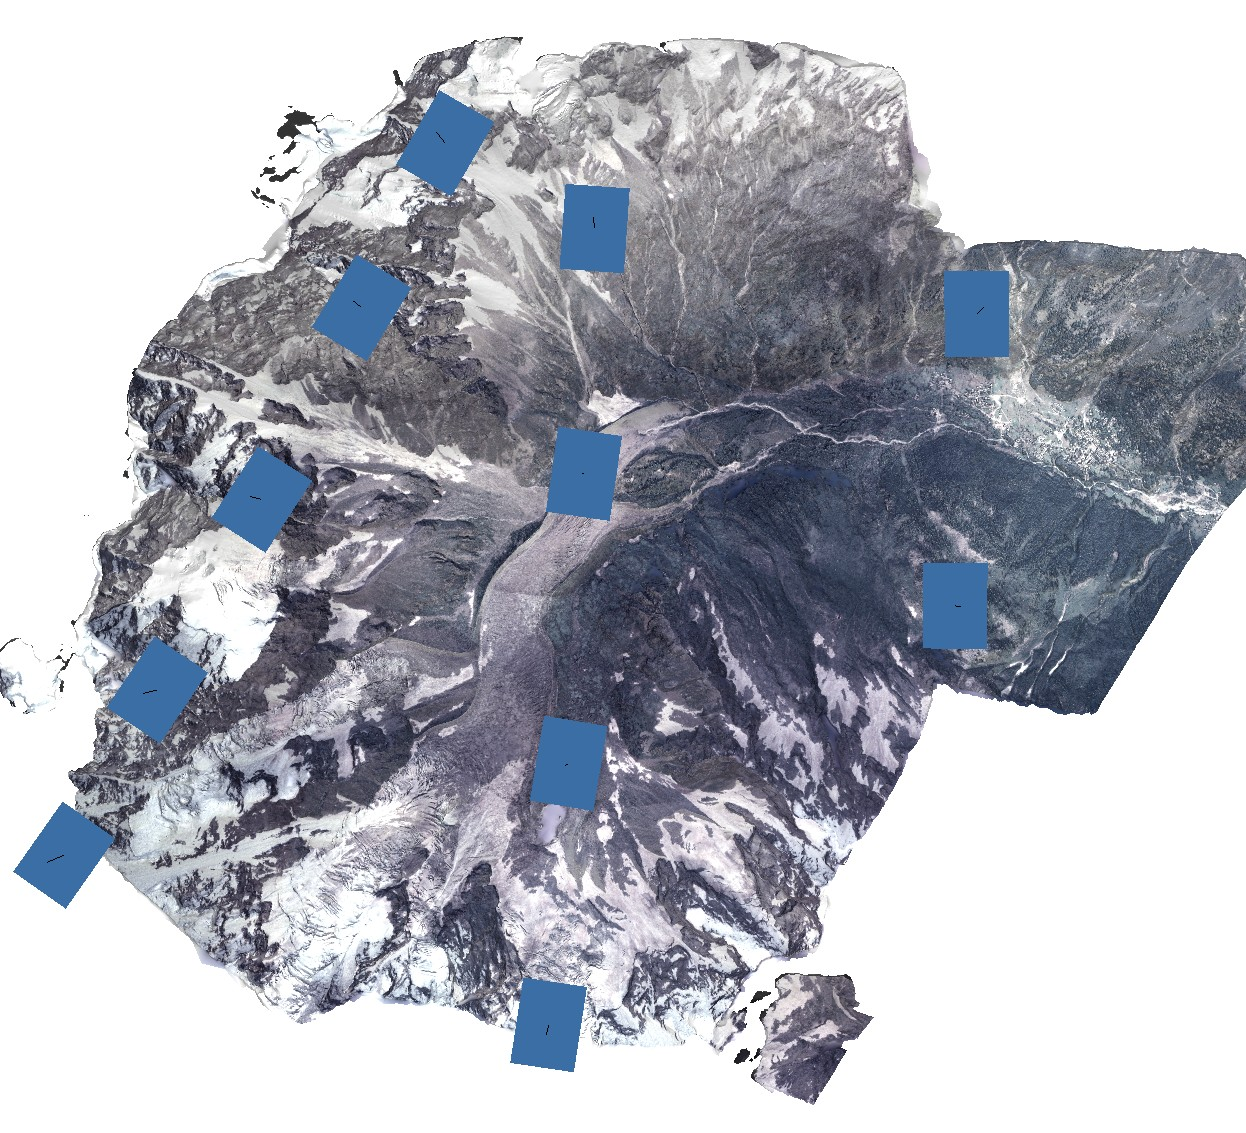
\includegraphics[height=5.5cm]{1977_block}
    } \quad
    \subcaptionbox{\label{fig:2:datasets_historical:1977_img}}{
        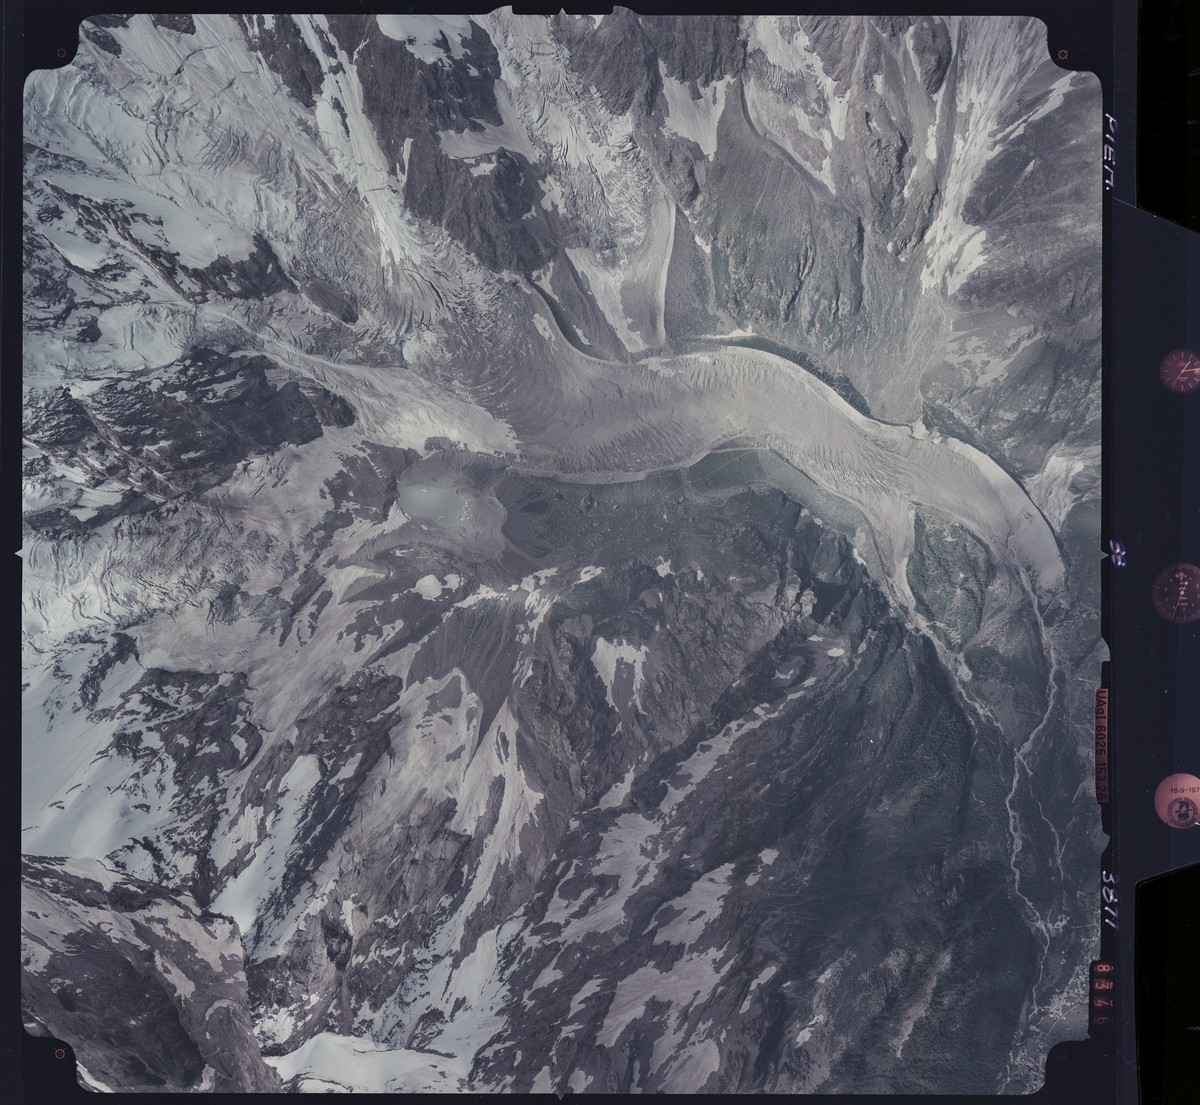
\includegraphics[height=5.5cm]{1977_img}
    } \\
    \subcaptionbox{\label{fig:2:datasets_historical:1991_block}}{
        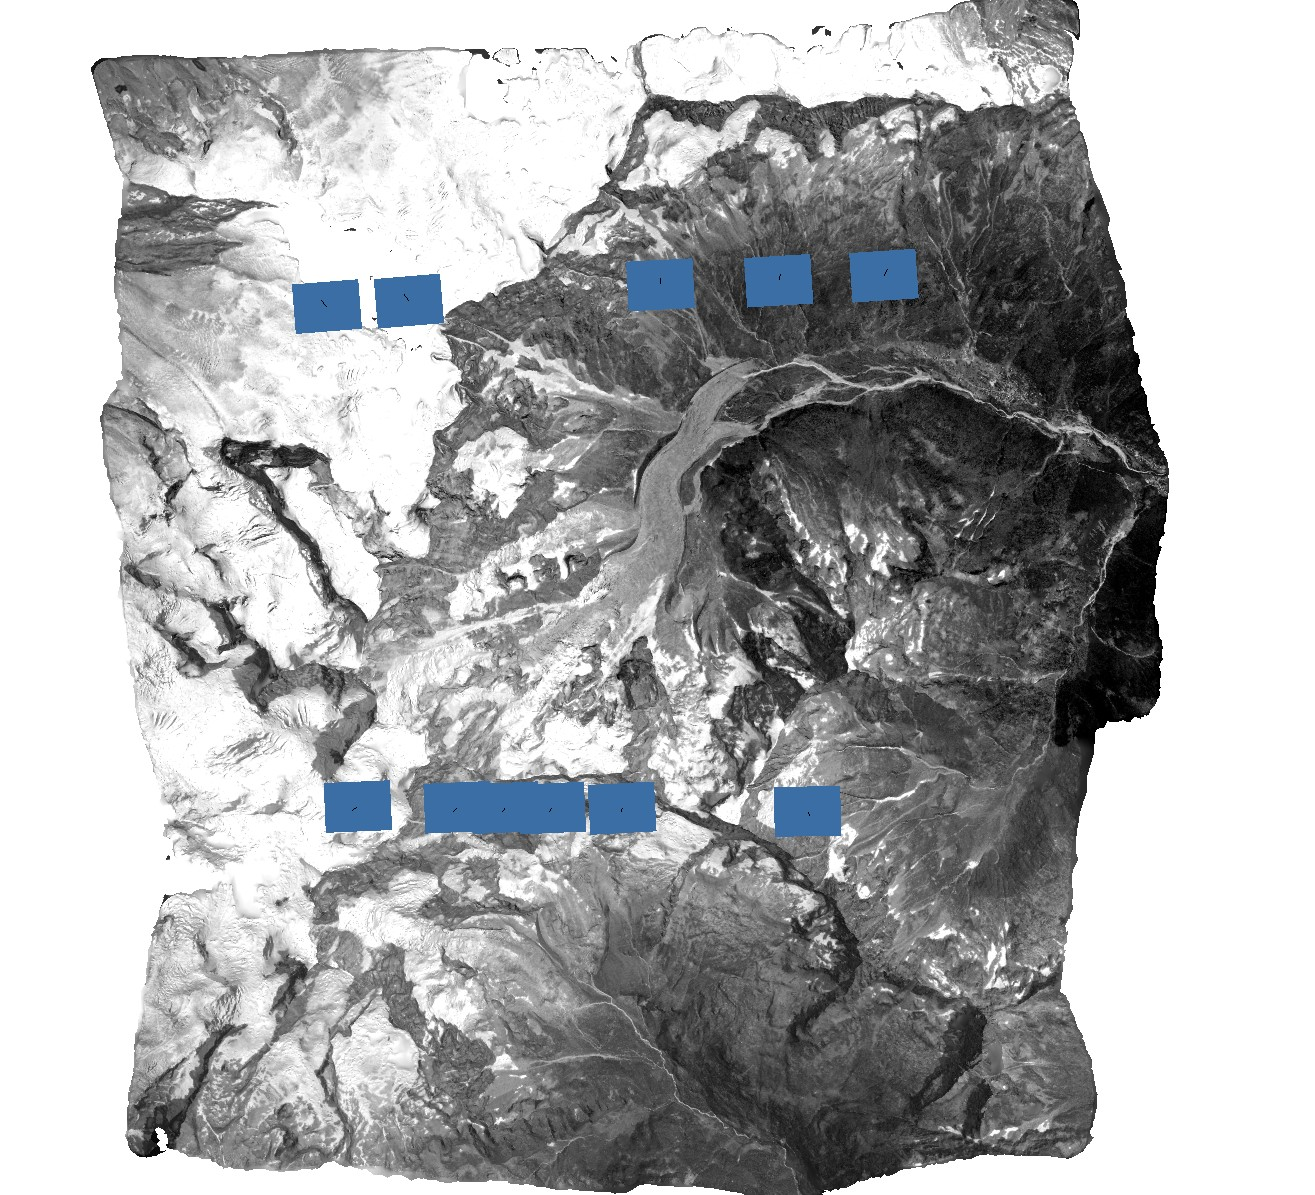
\includegraphics[height=5.5cm]{1991_block}
    } \quad
    \subcaptionbox{\label{fig:2:datasets_historical:1991_img}}{
        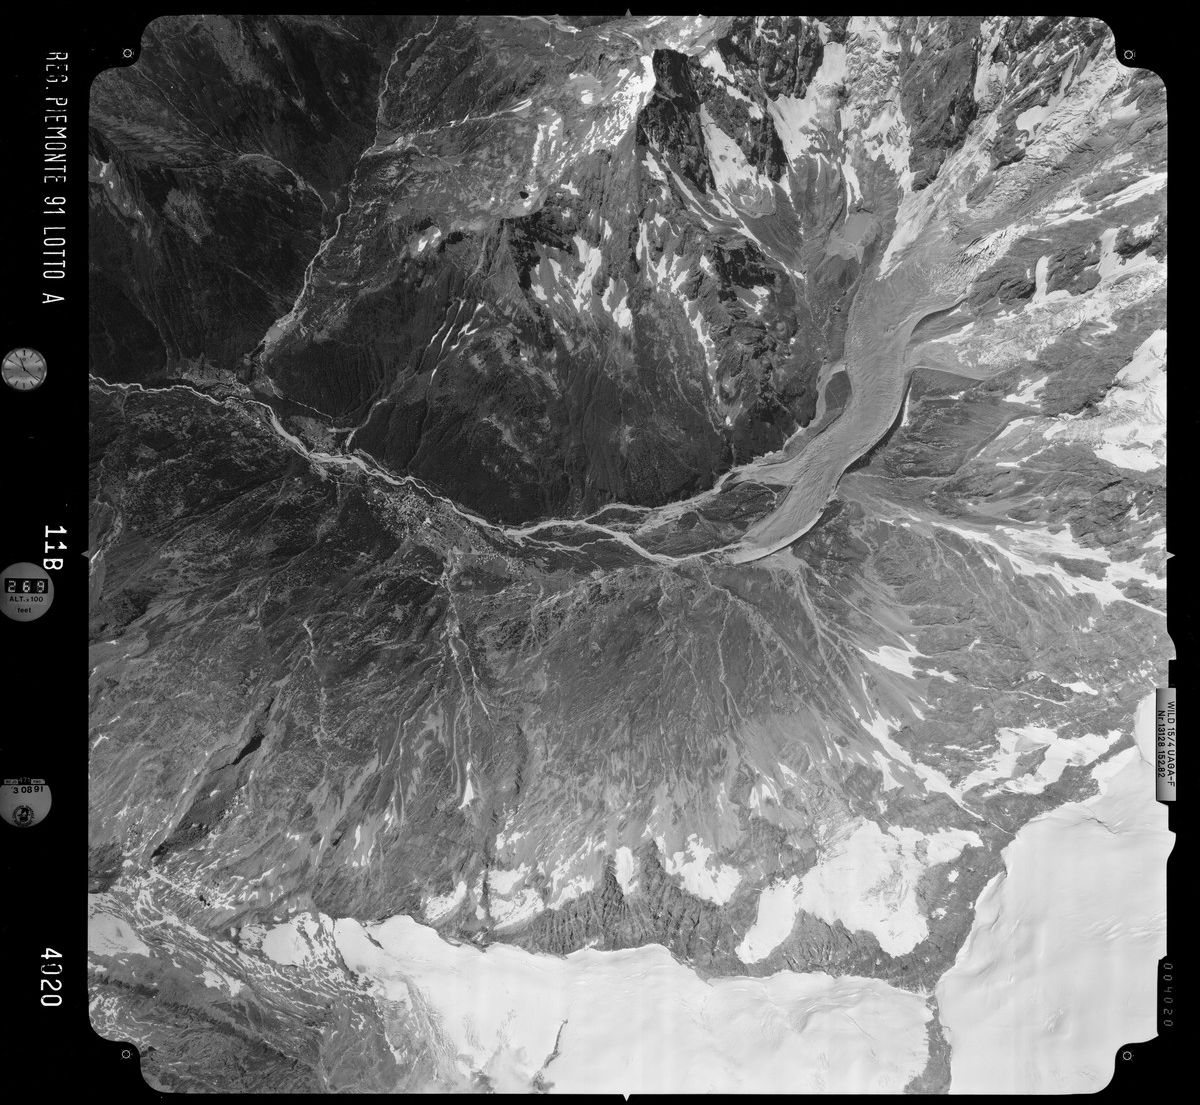
\includegraphics[height=5.5cm]{1991_img}
    } \\
    \subcaptionbox{\label{fig:2:datasets_historical:2001_block}}{
        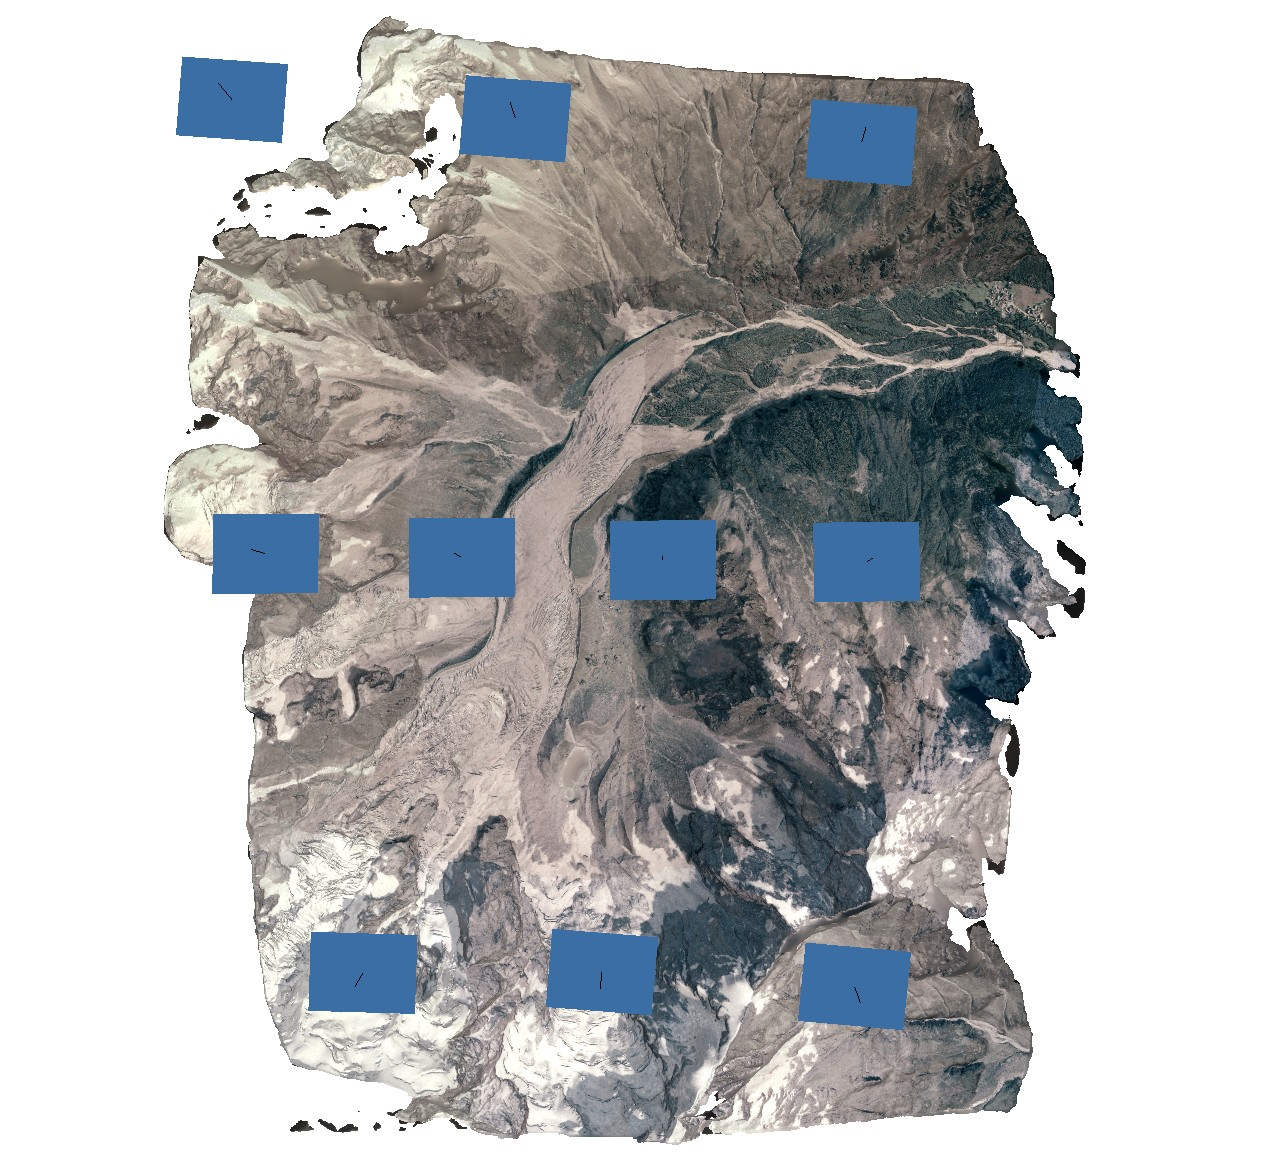
\includegraphics[height=5.5cm]{2001_block}
    } \quad
    \subcaptionbox{\label{fig:2:datasets_historical:2001_img}}{
        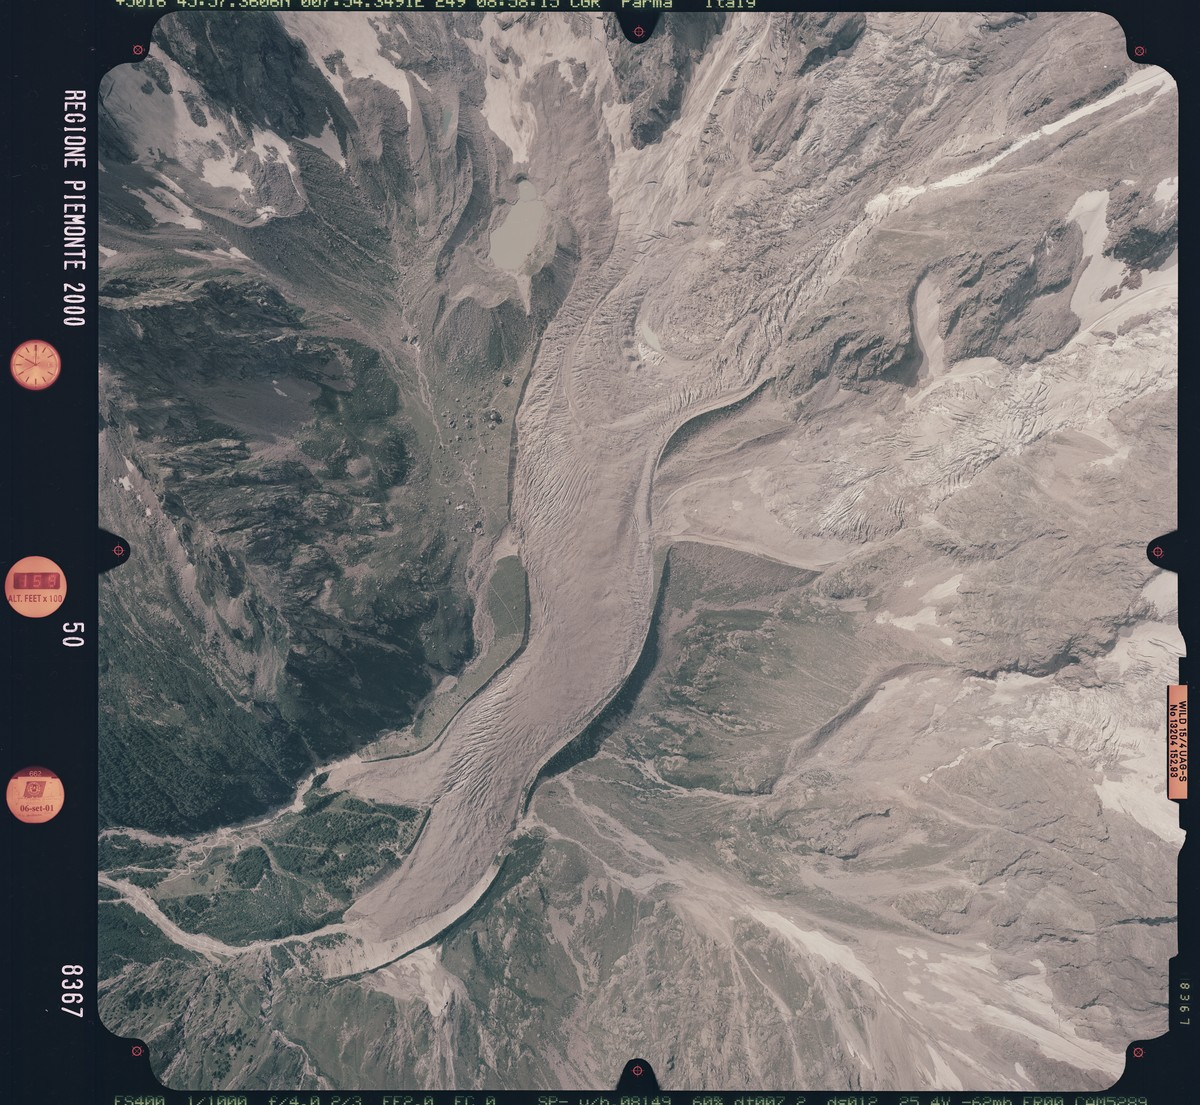
\includegraphics[height=5.5cm]{2001_img}
    } \\
    \caption{Historical datasets of \textbf{a,b} 1977, \textbf{c,d} 1991, \textbf{e,f} and 2001. A picture depicting the image acquisition geometry (left) and a sample of the scanned analog images (right) is presented for each dataset.}
    \label{fig:2:datasets_historical}
\end{figure}

The earliest dataset considered in the study was acquired by CGR S.p.A. on 16/09/1977
with an analog photogrammetric camera Wild RC10, equipped with a 15 UAG I lens with
a focal length of 153.26 mm. 
The flight consisted of three stripes performed at an average altitude of 5600 m a.s.l., with approximately 60\% along-flight overlap and transversal overlap varying from 30\% to 60\% because the stripes were not parallel. 
A total of 11 RGB images were acquired (\figref{fig:2:datasets_historical:1977_block}). 
Considering the average altitude of the glacier of \SI{2000}{\masl}, the scale of the images was about 1:23,000, leading to an average ground sample distance (GSD) of 0.5 m. 
The camera reference system was materialized on the film with four fiducial marks placed at the four corners of the image. As is visible in \figref{fig:2:datasets_historical:1977_img}, some of the fiducial marks were faded due to the aging of the films, but they were still identifiable in the digitalized images.

The 1991 survey was carried out on two different days: 03/08/1991 and 07/08/1991.
Eleven grayscale images were taken with an analog photogrammetric camera, a Wild RC20
equipped with a 15/4 UAGA F lens (focal length of 153.26 mm). The flight consisted of only
two stripes ((\figref{fig:2:datasets_historical:1991_block})), conducted at \SI{8200}{\masl} and \SI{8500}{\masl}, leading to an average
GSD for the images of about 0.9 m. The along-flight overlap was approximately between
70\% and 80\%, while the transversal overlap was about 50\%. As in the images of 1977, four
fiducial marks allowed for the definition of the camera reference system (\figref{fig:2:datasets_historical:1991_img}).

The most recent among the three historical datasets dates back to 2001. Images were
acquired with a film camera Wild RC30 equipped with a 15/4 UAG-S lens (focal length
of 153.928 mm). The flight consisted of three stripes acquired between 06/09/2001 and
11/09/2001, producing a total of ten RGB images with overlaps of ~70\% along flight and
~50\% in the transversal direction (\figref{fig:2:datasets_historical:2001_block}). The two external stripes were conducted at an
altitude of about \SI{6100}{\masl}, while the central one was conducted at a lower altitude of
about \SI{4800}{\masl}, for an average of \SI{5800}{\masl}. The mean scale of the images was 1:23,000, producing a GSD of 0.5 m, comparable to that of the 1977 flight. 
The camera reference frame was materialized by eight fiducial marks, well identifiable on the digitalized images (\figref{fig:2:datasets_historical:1977_img}).

Historical aerial images were digitalized using a photogrammetric scanner PhotoScan2000, developed by Z/I Imaging and Carl Zeiss, capable of scanning analog film rolls. 
The images were digitalized by CGR S.p.A. with a resolution of 21 µm/px, producing eight-bit TIF 
images with dimensions of \qtyproduct{12 098 x 11 144}{\pixel}. 
To assess the quality of the digitalized images, the actual pixel size was computed as the average ratio of the distance (in millimeters) between the fiducial marks with the corresponding distance in pixels. 
The estimated pixel size was \qtyproduct{21 x 21}{\micro\meter} for each dataset, with a standard deviation of about three orders of magnitude less, in agreement with the technical scanner specifications.

\begin{figure}[ht]
    \centering
    \subcaptionbox{\label{fig:2:datasets_digital:2009_block}}[.35\textwidth]{
        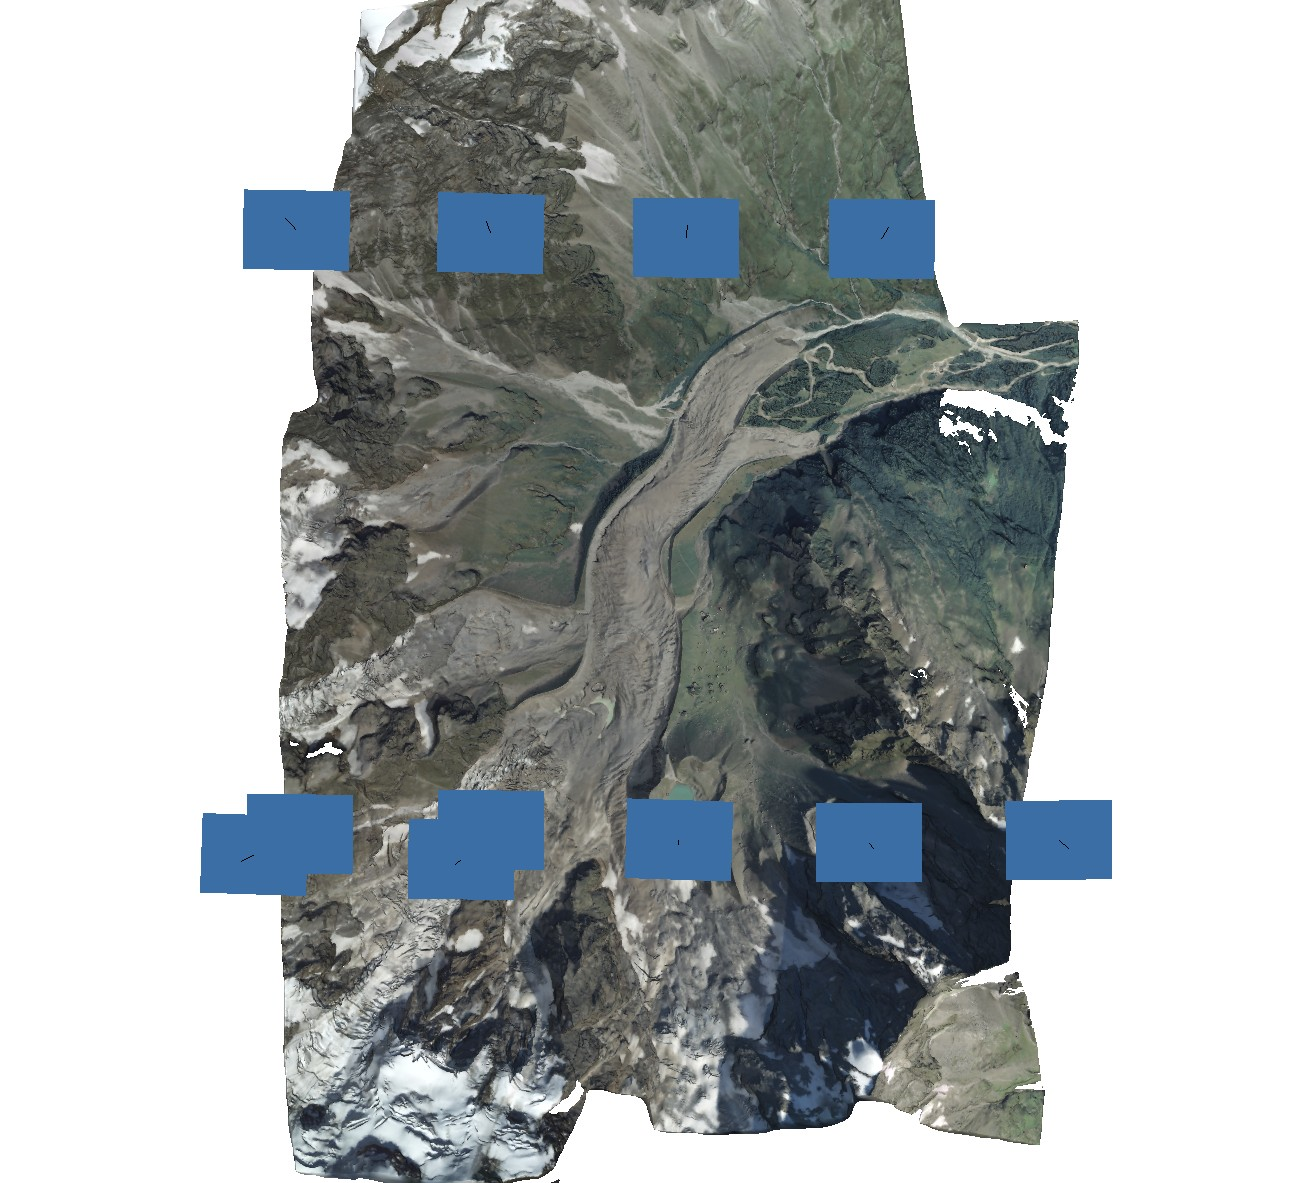
\includegraphics[height=5cm]{2009_block}
    } \quad
    \subcaptionbox{\label{fig:2:datasets_digital:2009_img}}[.6\textwidth]{
        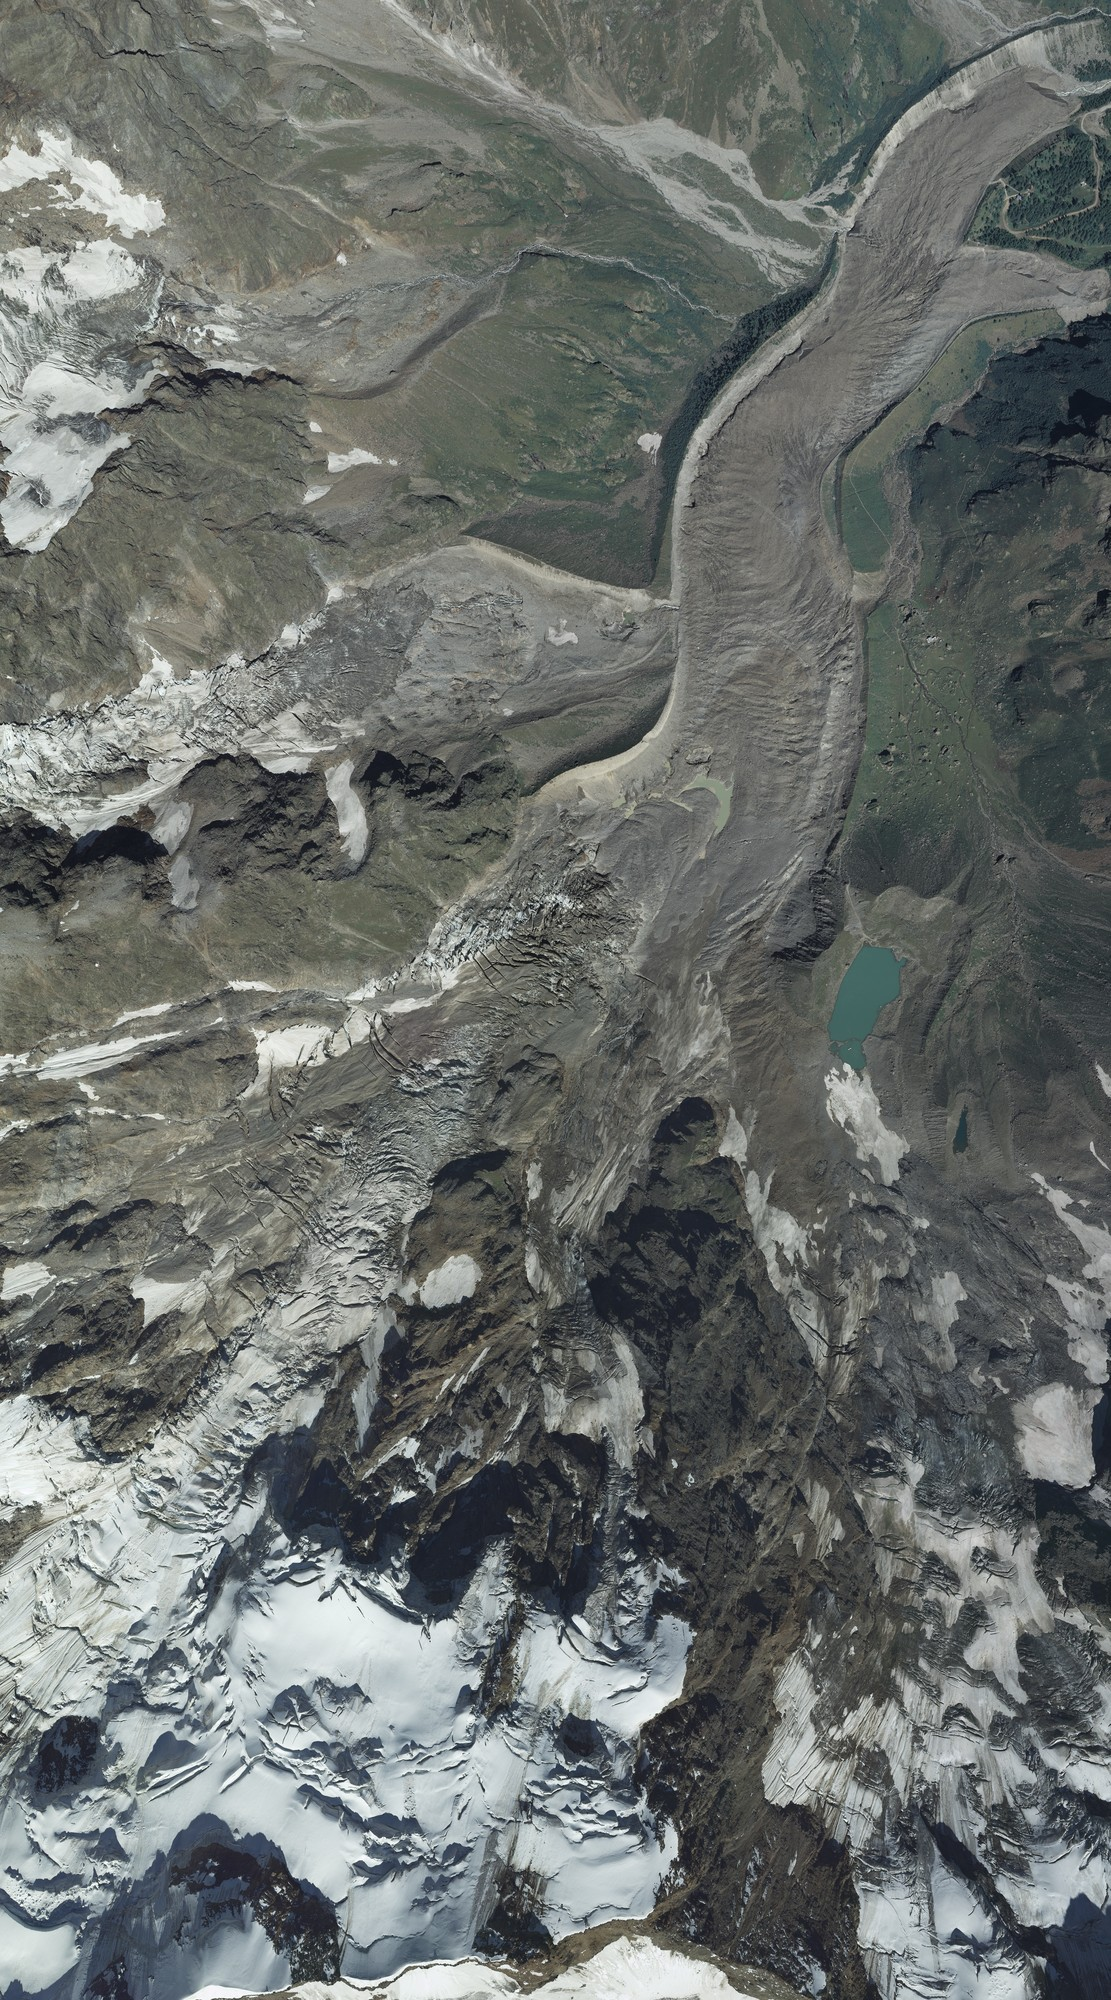
\includegraphics[height=5cm]{2009_img}
    } \\
    \subcaptionbox{\label{fig:2:datasets_digital:2019_block}}[.35\textwidth]{
        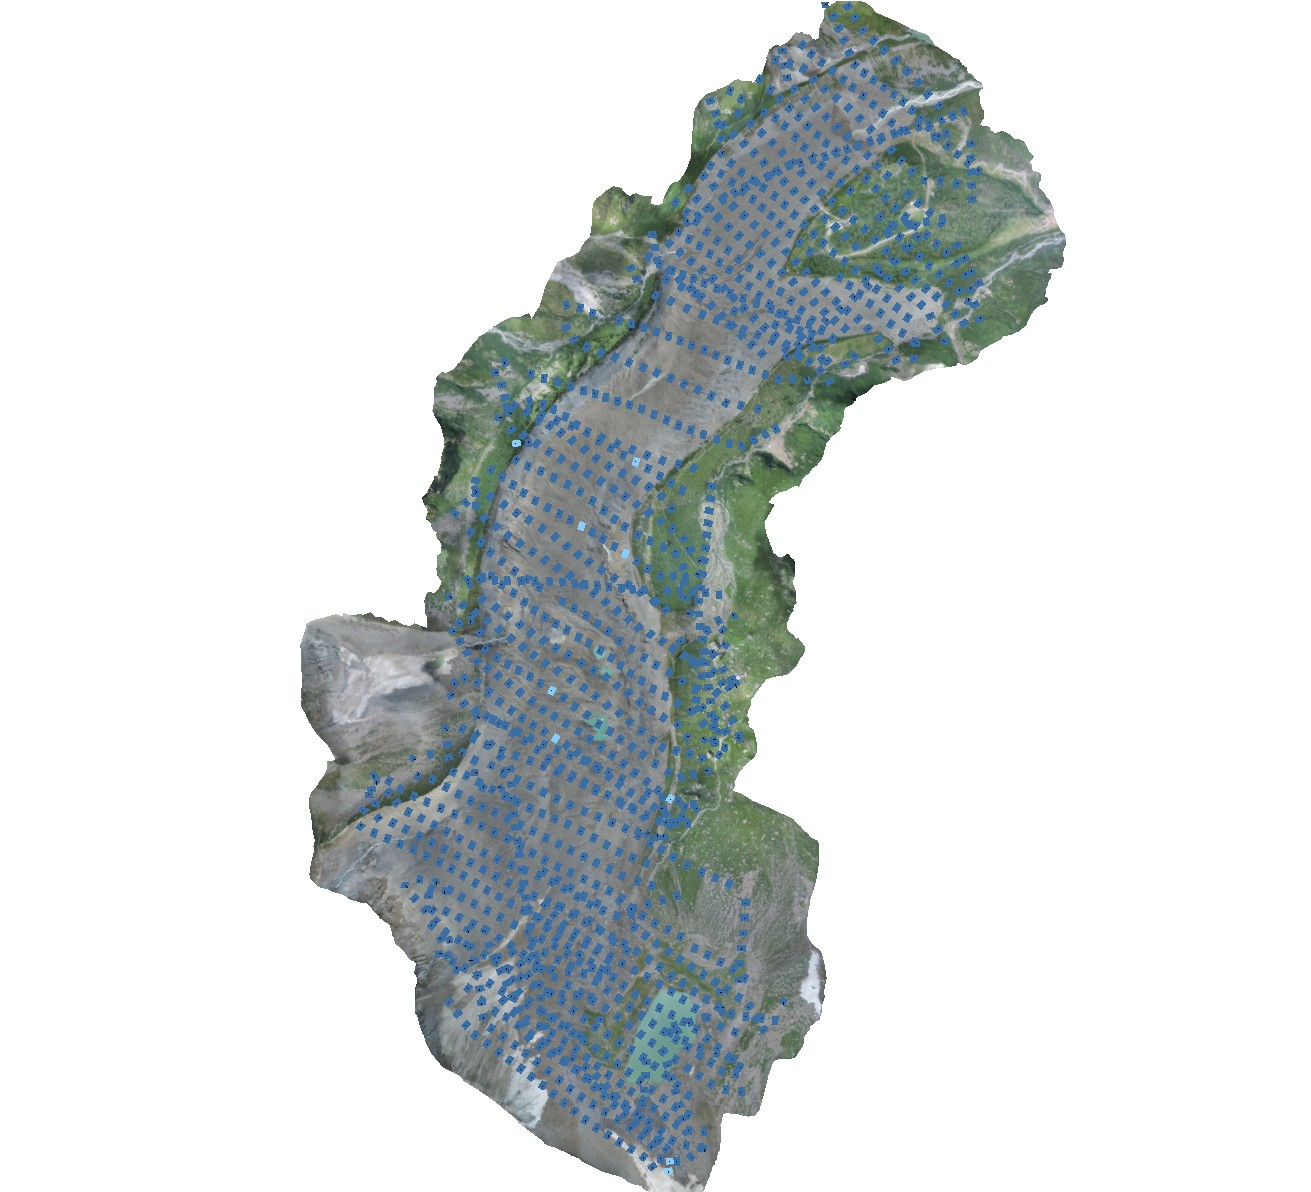
\includegraphics[height=5cm]{2019_block}
    } \quad
    \subcaptionbox{\label{fig:2:datasets_digital:2019_img}}[.6\textwidth]{
        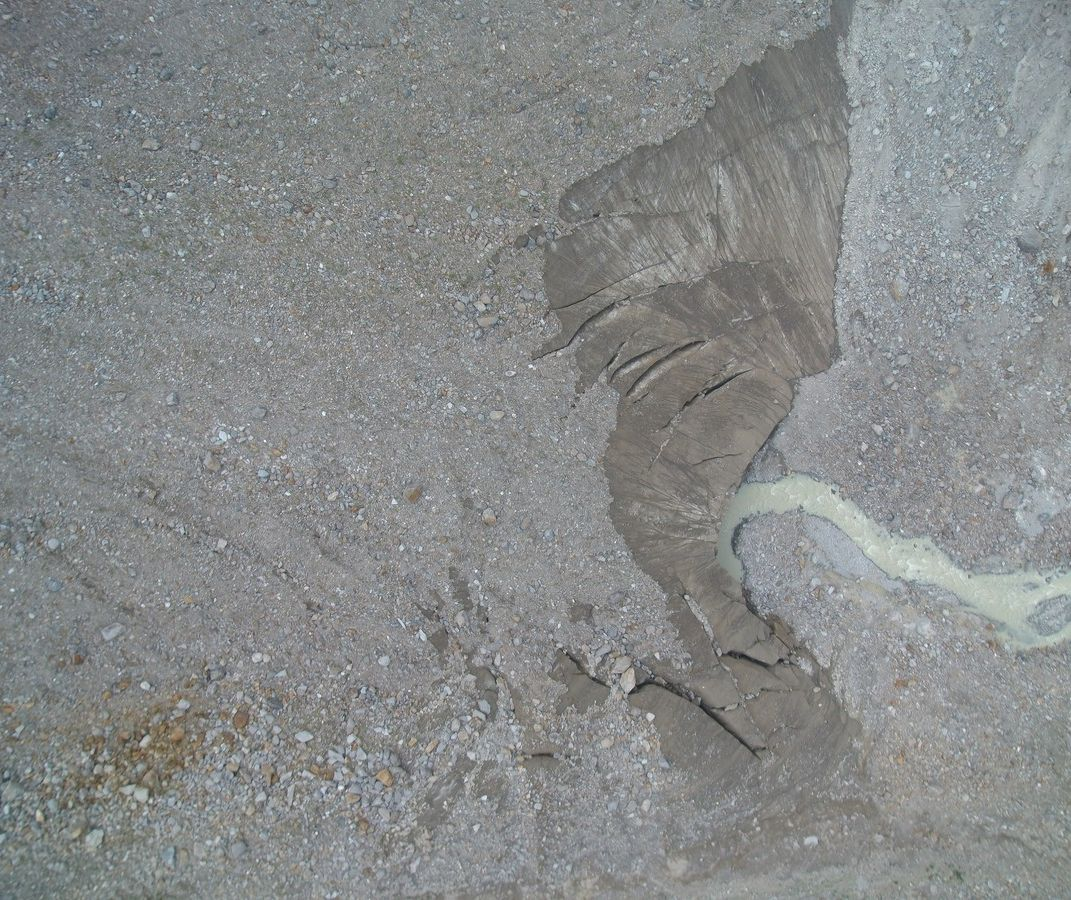
\includegraphics[height=5cm]{2019_img}
    } \\
    \caption{Digital datasets of \textbf{a,b} 2009 (aerial), \textbf{c,d} 2019 (UAV). For each dataset, a picture depicting the image acquisition geometry (left) and a sample image (right) is presented.}
    \label{fig:2:datasets_digital}
\end{figure}

\subsection{Digital aerial dataset of 2009}

In October 2009, CGR S.p.A. flew over Belvedere Glacier for mapping purposes. 
This time, a digital photogrammetric camera was employed.
A Z/I-Imaging DMC camera equipped with a 120 mm focal length lens and a CCD
sensor with a pixel size of 12 µm × 12 µm, acquiring RGB digital images at a resolution of 7680 × 13,824 pixels, was mounted on an airplane. 
Eleven images with along-flight and transversal overlaps of 70\% and 50\%, respectively, were gathered along two stripes with altitudes between 5600 and 6000 m a.s.l~\figref{fig:2:datasets_digital}a-b). 
The average image scale was 1:32,000, and the GSD was 0.4 m.

\subsection{Digital UAV dataset of 2019}

The authors gathered images from the latest dataset during fieldwork on the Belvedere Glacier between 29/07/2019 and 02/08/2019~\citep{Ioli2022}. 
A fixed-wing UAV Parrot Disco was adapted to carry a low-cost and lightweight action
camera, a HawkEye Firefly 8S. 
The action camera was equipped with a 12 Mpx 1/2.3" CMOS sensor, with a pixel size of 1.34 µm × 1.34 µm and a focal length of 3.8 mm (90◦ field of view). 
The flights were conducted at an average height of 120 m a.g.l. (above ground level), in agreement with Italian UAV regulations, and images were taken with longitudinal and transversal overlap of 80\% and 60\%, respectively (except for a small portion in the middle of the glacier with a slightly smaller transversal overlap of ~50\%; see \figref{fig:2:datasets_digital:2019_block}).
Therefore, the average image scale was approximately 1:32,000, and the GSD was 5 cm, one order of magnitude smaller than the aerial datasets. 
Because of UAV technical limitations, the survey area was restricted to the glacier body only, and five flights with the fixed-wing UAV were performed (\figref{fig:2:datasets_digital:2019_block})


\subsection{GNSS Survey for Block Georeferencing}

To constrain the UAV photogrammetric block from 2019, 36 squared targets, consisting
of 50 cm × 50 cm polypropylene sheets with high color contrast, were deployed over the
survey area, anchored to large rocks on both the glacier and the moraines. Among the
36 targets, 26 were used as ground control points (GCPs) and 10 as control points (CPs).
The targets were measured on the field with a dual frequency (L1/L2) geodetic quality
GNSS receiver Leica Viva GS14. Because a GSM internet connection was available in the lower
part of the glacier, the targets were measured in nRTK relative to the HxGN SmartNet
network of permanent stations. All the points measured in nRTK were occupied for ~10 s
with a 1 Hz acquisition rate. In the upper part of the glacier, where nRTK was not possible,
the targets were measured by static positioning. For each of those points, carrier-phase
raw observations were logged for a timespan of \SI{\sim 10}{\minute} (1 Hz sampling rate).
These were postprocessed relative to a local master station (Leica GPS1200) placed 
over a target next to the Zamboni–Zappa hut (2070 m a.s.l.). 
Coordinates of the master station were repeatedly measured in different years, with both
static and nRTK measurements, and accuracy on the order of 0.5 cm in planimetry and 2 cm 
in height was obtained. 
GNSS observations were post-processed with Leica Infinity software (version 3.2.0) in the official Italian reference system ETRF2000 at epoch 2008.0. 
The resulting accuracies of the GCPs' coordinates were 1.5 cm in planimetry and 3 cm in height in terms of average RMSE.

\section{Methodology}\label{sec:2:methods}

\subsection{SfM-MVS}

The photogrammetric software Agisoft Metashape (version 1.7.2) was employed for image orientation and model reconstruction of all the datasets. A sketch of the following
workflow is provided in \figref{fig:2:workflow}

\begin{figure}
    \centering
    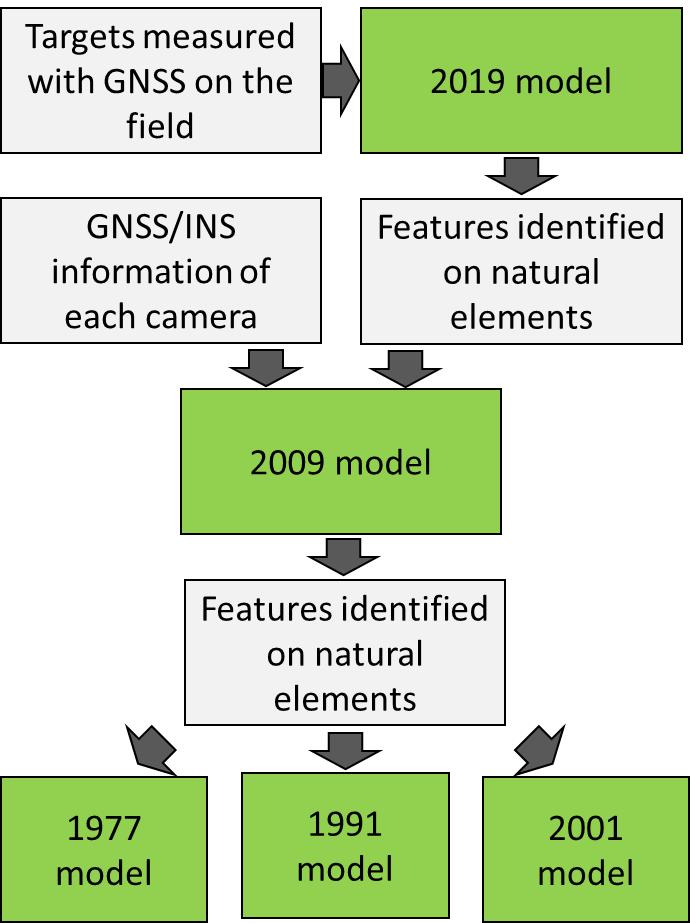
\includegraphics[width=0.5\textwidth]{workflow}
    \caption{Workflow for the reconstruction of models and their spatial alignment in a common reference frame}
    \label{fig:2:workflow}
\end{figure}

\begin{figure}
    \centering
    \subcaptionbox{\label{fig:2:gcp:historical}}[.32\textwidth]{
        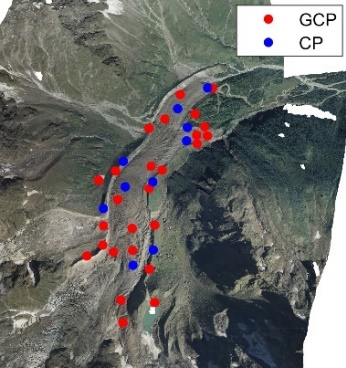
\includegraphics[height=5.3cm]{gcp_historical}
    } \hspace{1mm}
    \subcaptionbox{\label{fig:2:gcp:2009}}[.32\textwidth]{
        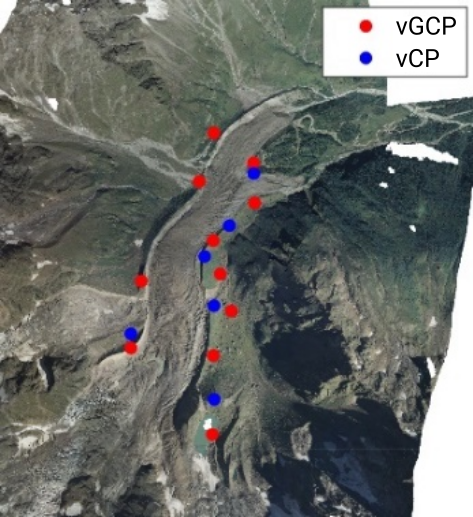
\includegraphics[height=5.3cm]{gcp_2009}
    }
    \subcaptionbox{\label{fig:2:gcp:2019}}[.32\textwidth]{
        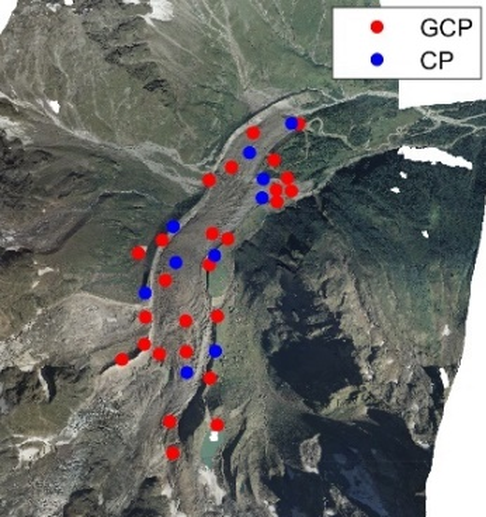
\includegraphics[height=5.3cm]{gcp_2019}
    } 
    \caption{Sketches of the GCPs and CPs locations; (a) 1977, 1991 and 2001 surveys; (b) 2009 survey; (c) 2019 survey.}
    \label{fig:2:gcp}
\end{figure}

Concerning the most recent UAV survey from 2019, the 1486 images were oriented by traditional aerial triangulation based on 26 targets spread over the survey
\figref{fig:2:gcp} area used as GCPs in the Bundle Block Adjustment (BBA).
The GCPs were manually collimated on the images.
A collimation accuracy of 1 px was assumed as the a priori standard deviation of the observations within the BBA. 
Tie Points (TPs) were automatically detected and matched by Metashape on full-resolution images.
Camera Internal Orientation (IO) parameters of the Hawkeye Firefly 8S action camera were
estimated during the BBA by self-calibration. 
To this end, approximated IO parameters were precalibrated using a traditional checkerboard. 
However, these initial values were adjusted for each flight because of the internal instability of the camera and thanks to the high density of the GCPs available.

Regarding the 2009 digital dataset, the Z/I-Imaging DMC system included high-precision GNSS/INS instrumentation, providing the camera External Orientation (EO) \citep{Hinz2001}. 
The coordinates of the camera projection centers were provided with an accuracy of 30 cm, while the camera attitude angles had an accuracy of 8 mgon for roll and pitch angles and 10 mgon for yaw \citep{Forlani_pinto2001}.
To improve the quality of the photogrammetric block within a small area such as that of Belvedere Glacier, 11 features identifiable on the images (e.g., sharp rocks) were used as GCPs. 
Their coordinates were retrieved from the 2019 model, which has a significantly higher spatial resolution (\tabref{tab:2:camera_summary}). 
EO of the images was estimated through Assisted Aerial Triangulation (AAT) \citep{ioli2021_lowcost_dgps}. 
The BBA was solved by combining GNSS/INS information with TPs automatically detected by the software and 11 GCPs manually collimated on the images. 
The quality of the photogrammetric model was assessed by employing 6 Check Points (CP), which were not used to solve the BBA. 

\begin{figure} [ht]
    \centering
    \subcaptionbox{\label{fig:2:gcp_examples:artificial}}[\textwidth]{
        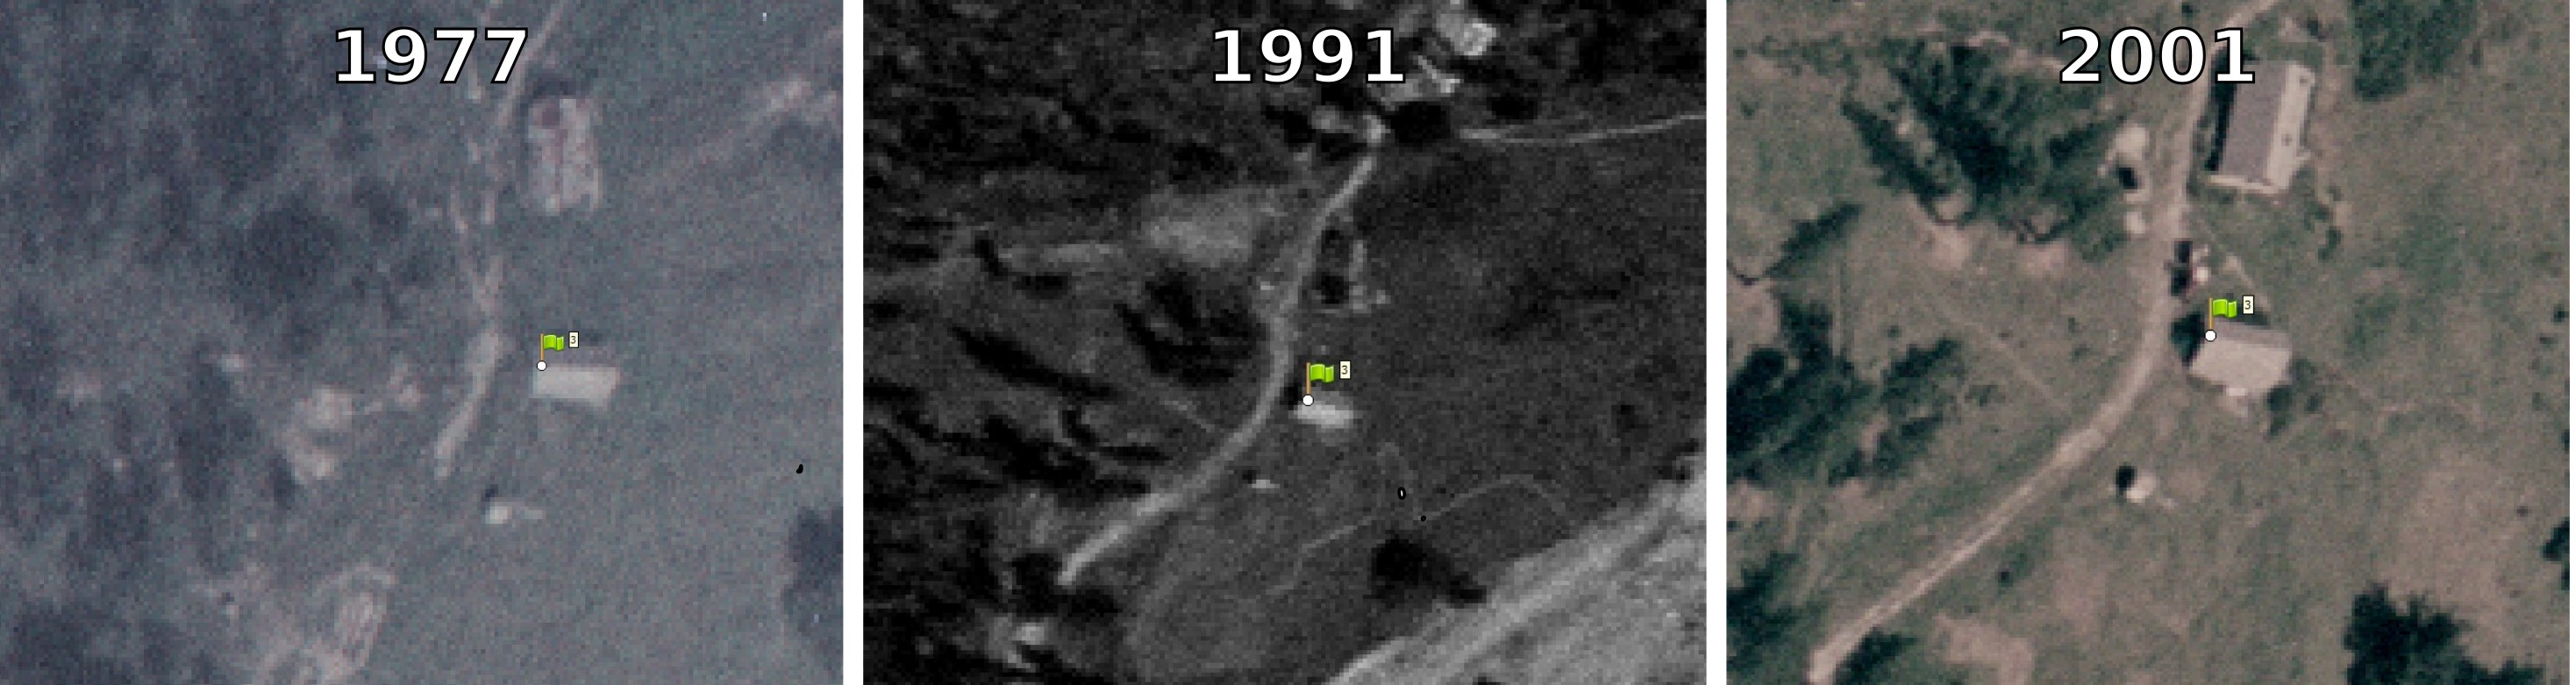
\includegraphics[width=\textwidth]{artificial_gcps}
    } \\
    \subcaptionbox{\label{fig:2:gcp_examples:natural}}[\textwidth]{
        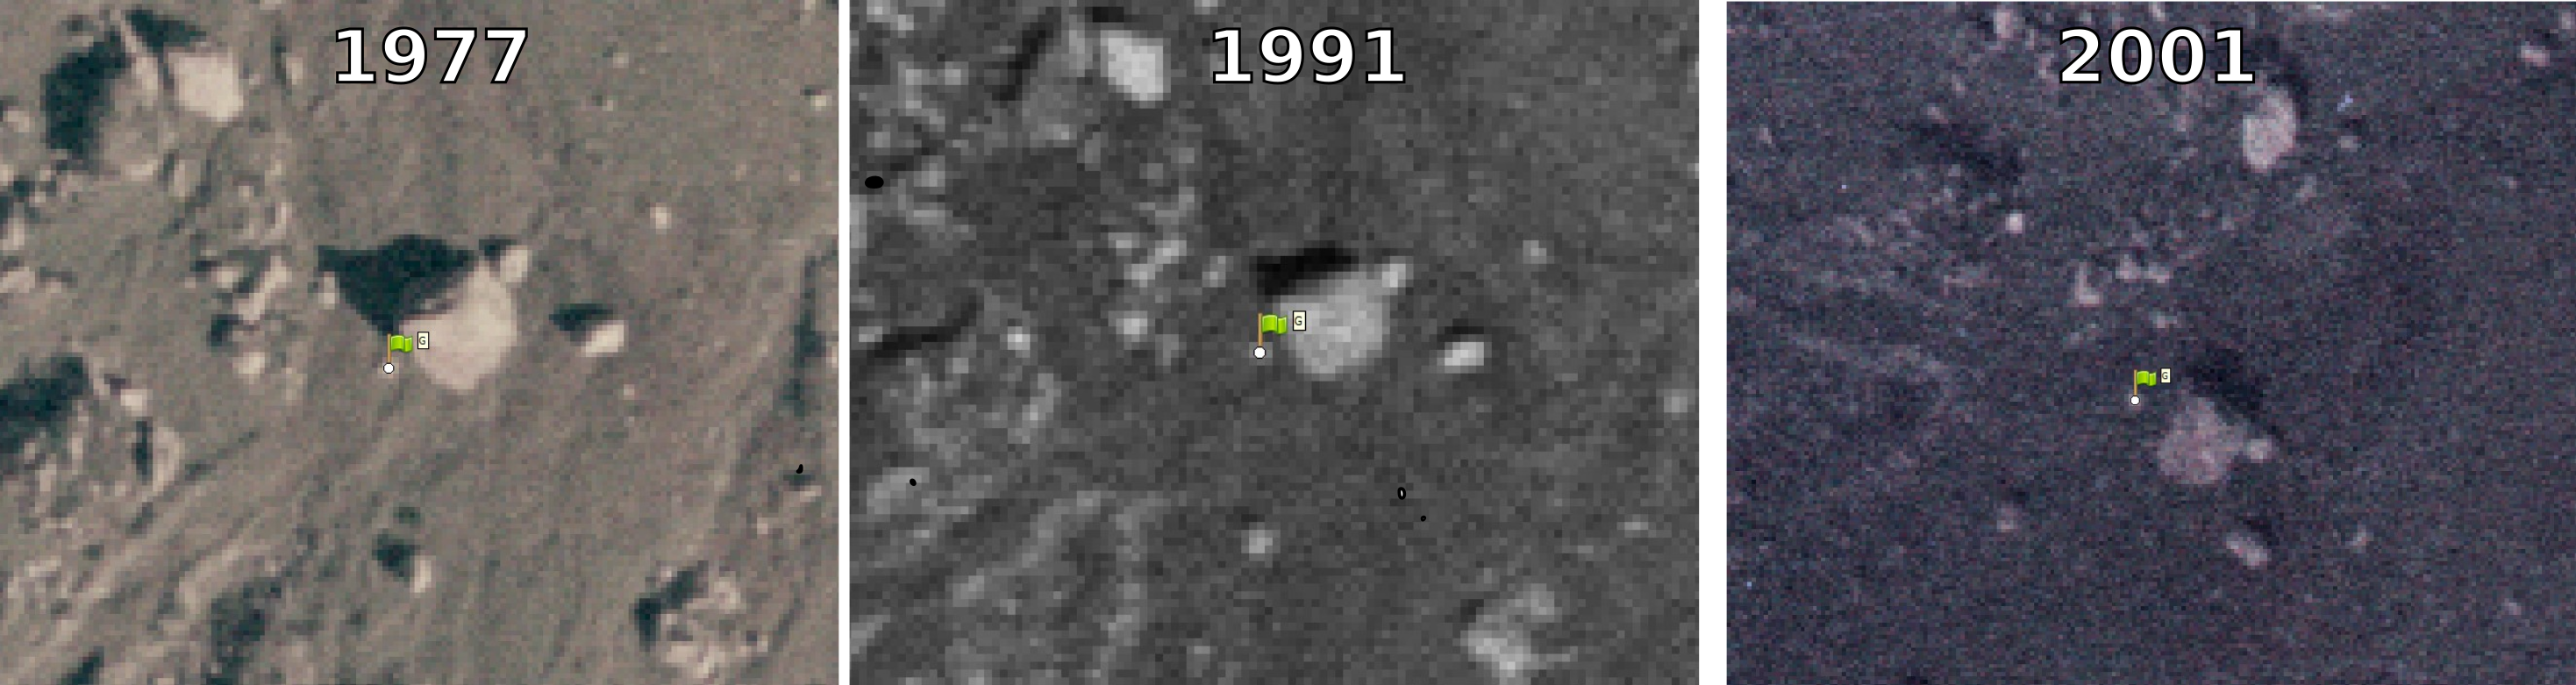
\includegraphics[width=\textwidth]{natural_gcps}
    }
    \caption{Examples of points chosen as GCPs or CPs: (a) artificial features in 1977, 1991, and 2001 aerial images, respectively; (d) natural features in 1977, 1991, and 2001 aerial images, respectively.}
    \label{fig:2:gcp_examples}
\end{figure}

After the digitalization, the three historical datasets were oriented by aerial triangulation based on the 2009 block. The coordinates of nine GCPs (marked with numbers 1 to 9 in \figref{fig:2:gcp}) and eight CPs (marked with letters A to H), well distributed over the whole area, were retrieved from the aerial images acquired with the DMC digital photogrammetry system.
Points such as buildings edges, corners, sharp rocks along the glacier moraines, and particular morphological patterns that remained reasonably unchanged over time were selected in such a way as to be clearly identified in most of the four datasets (1977, 1991, 2001, and 2009), as shown in \figref{fig:2:gcp_examples}).
Note that it was not always possible to identify the same point in all four datasets because of the different image scales, different image quality (e.g., RGB versus grayscale images), or changes in the morphology over 30 years. Therefore, if one point was not visible in one dataset, another was searched nearby. To clarify, if one point (e.g., Point 2) was not found in images from 1991, then another feature, named Point 2b, was searched for close to the original location of Point 2 in the 2009 images and used as GCP for the 1991 dataset. However, in the statistics, Points 2 and 2b were considered one point because of their spatial proximity.
The GCPs used to solve the BBA of the three historical datasets were properly weighted with their variance. An accuracy of 0.75 px was assumed as the collimation accuracy for a human operator dealing with high-quality digital images such as those from 2009. This assumption was confirmed by the image reprojection error of the manually collimated points, which was always smaller than one pixel. Therefore, an a priori accuracy of 0.3 m was given to the GCPs in the three datasets from 1977, 1991, and 2001.

Concerning the camera interior orientation, the three analog cameras were calibrated in the laboratory by the producer, and calibration certificates were available. 
Therefore, the calibrated focal length and the principal point coordinates were provided as initial values in the BBA. 
These were then adjusted based on the GCPs using a self-calibration procedure \citep{jacobsen2004issues}. Additionally, two radial (k1 and k2) and tangential (p1 and p2) distortion parameters were estimated to correct the lens distortions of the photogrammetric cameras and the distortion introduced by external factors, e.g., the deterioration of the films over the years.

After BBA, dense point clouds (PCs), orthophotos, and DSMs were computed (a downscale factor of 2 was set to make the PCs more manageable) and used as a starting point for glacier analyses.

\subsection{Point cloud pre-processing}\label{sec:2:pcd_preproc}

The obtained point clouds referring to the different surveys required additional preprocessing to make them consistent for further analyses in terms of spatial resolution and coverage area.
The point clouds were initially rasterized by using CloudCompare (v2.12 alpha).
East–North gridded data with 0.5 m grid spacing were derived by averaging the height of the points inside each cell. 
Empty cells were initially filled with null values.

\begin{figure}[ht]
    \centering
    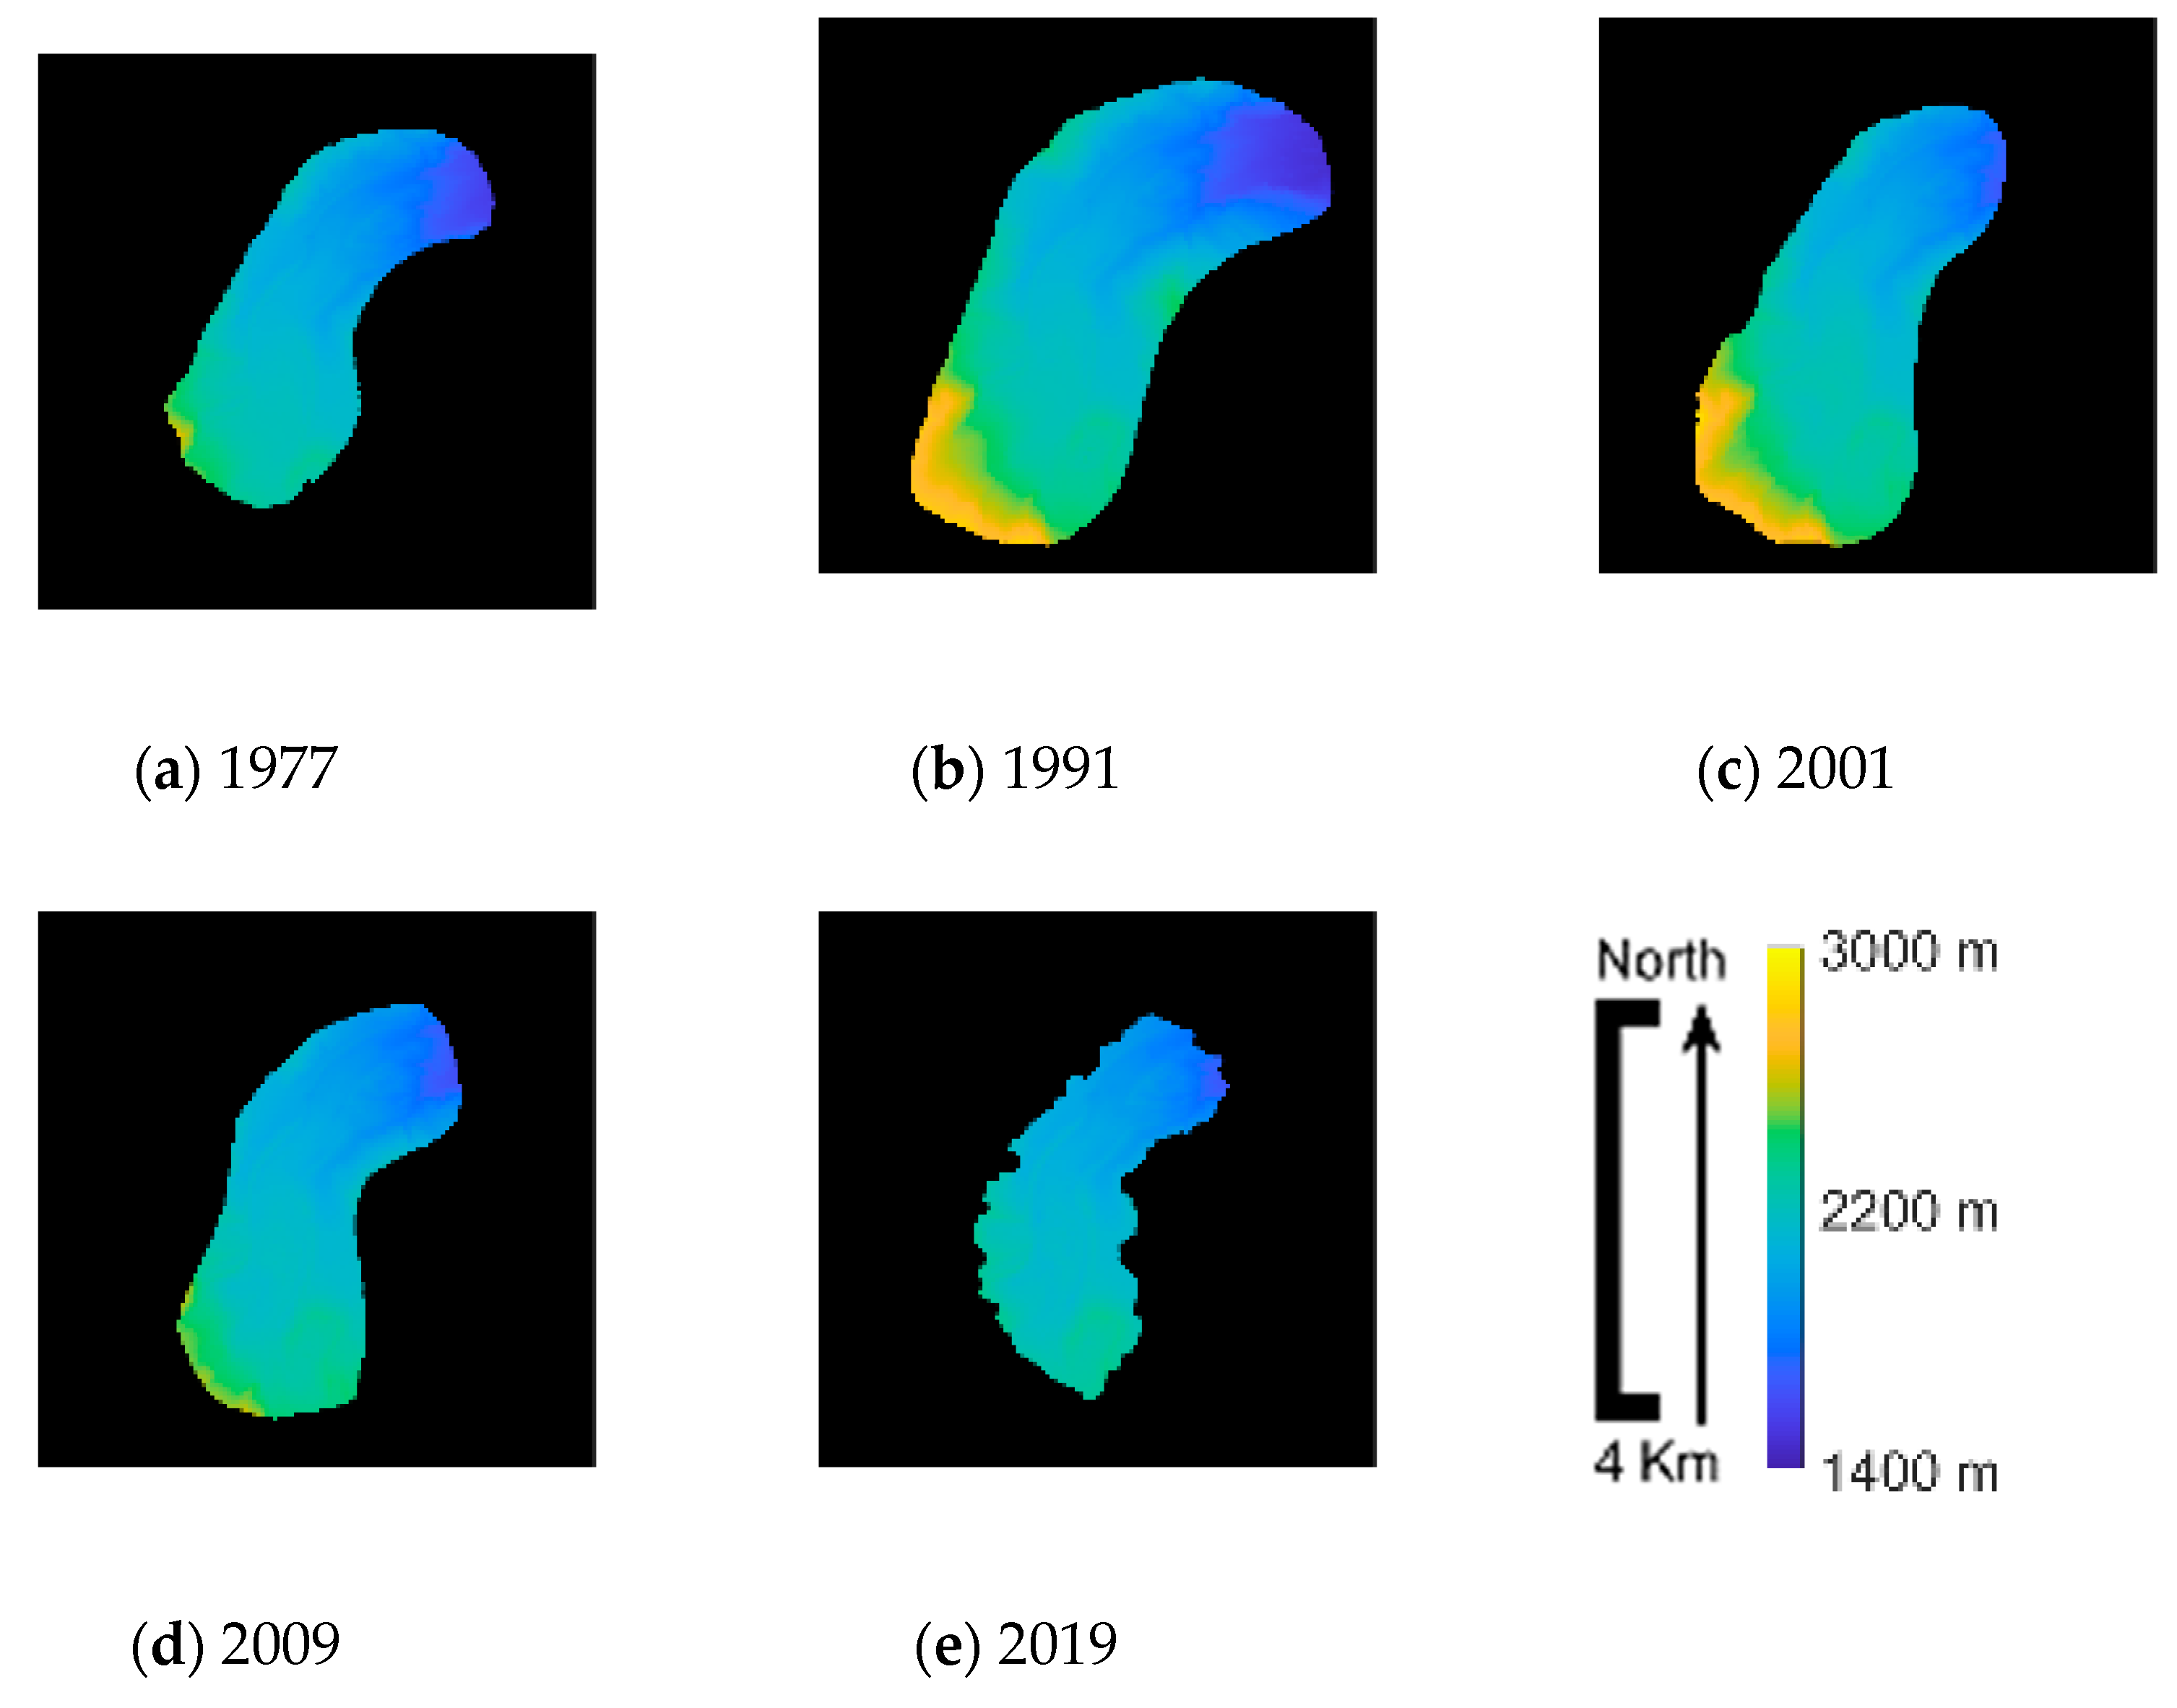
\includegraphics[width=0.90\textwidth]{pcd_rasterized.png}
    \caption{Interpolated gridded point clouds: (a) 1977; (b) 1991; (c) 2001; (d) 2009; (e) 2019.}
    \label{fig:2:pcd_rasterzed}
\end{figure}

The rasterized DSM was then manipulated in the MATLAB (R2020a) environment.
As the surveys' coverage areas are significantly different, the first step was automatically detecting the valid area for each photogrammetric DSM. 
This was done by first defining a binary mask with value 1 in correspondence with the DSM's non-null cells. 
The mask was then blurred by iterative convolutions with a kernel representing a circular box (10 m of radius) and assigning unitary value to resulting cells with values greater than 0 until no voids were present in the inner area.
A binary mask defining the valid surveyed area was obtained by applying the converse procedure (i.e., blurring with the same kernel and assigning 0 to the resulting cells with values smaller than 1) for the same number of iterations.
Finally, empty cells of the initial rasterized DSM within the valid surveyed area were filled via triangulation-based bi-dimensional linear interpolation.
As a result, gridded point clouds at a consistent resolution of 0.5 m were obtained for all five surveys (\figref{fig:2:pcd_rasterzed}).

\begin{figure}[ht]
    \centering
    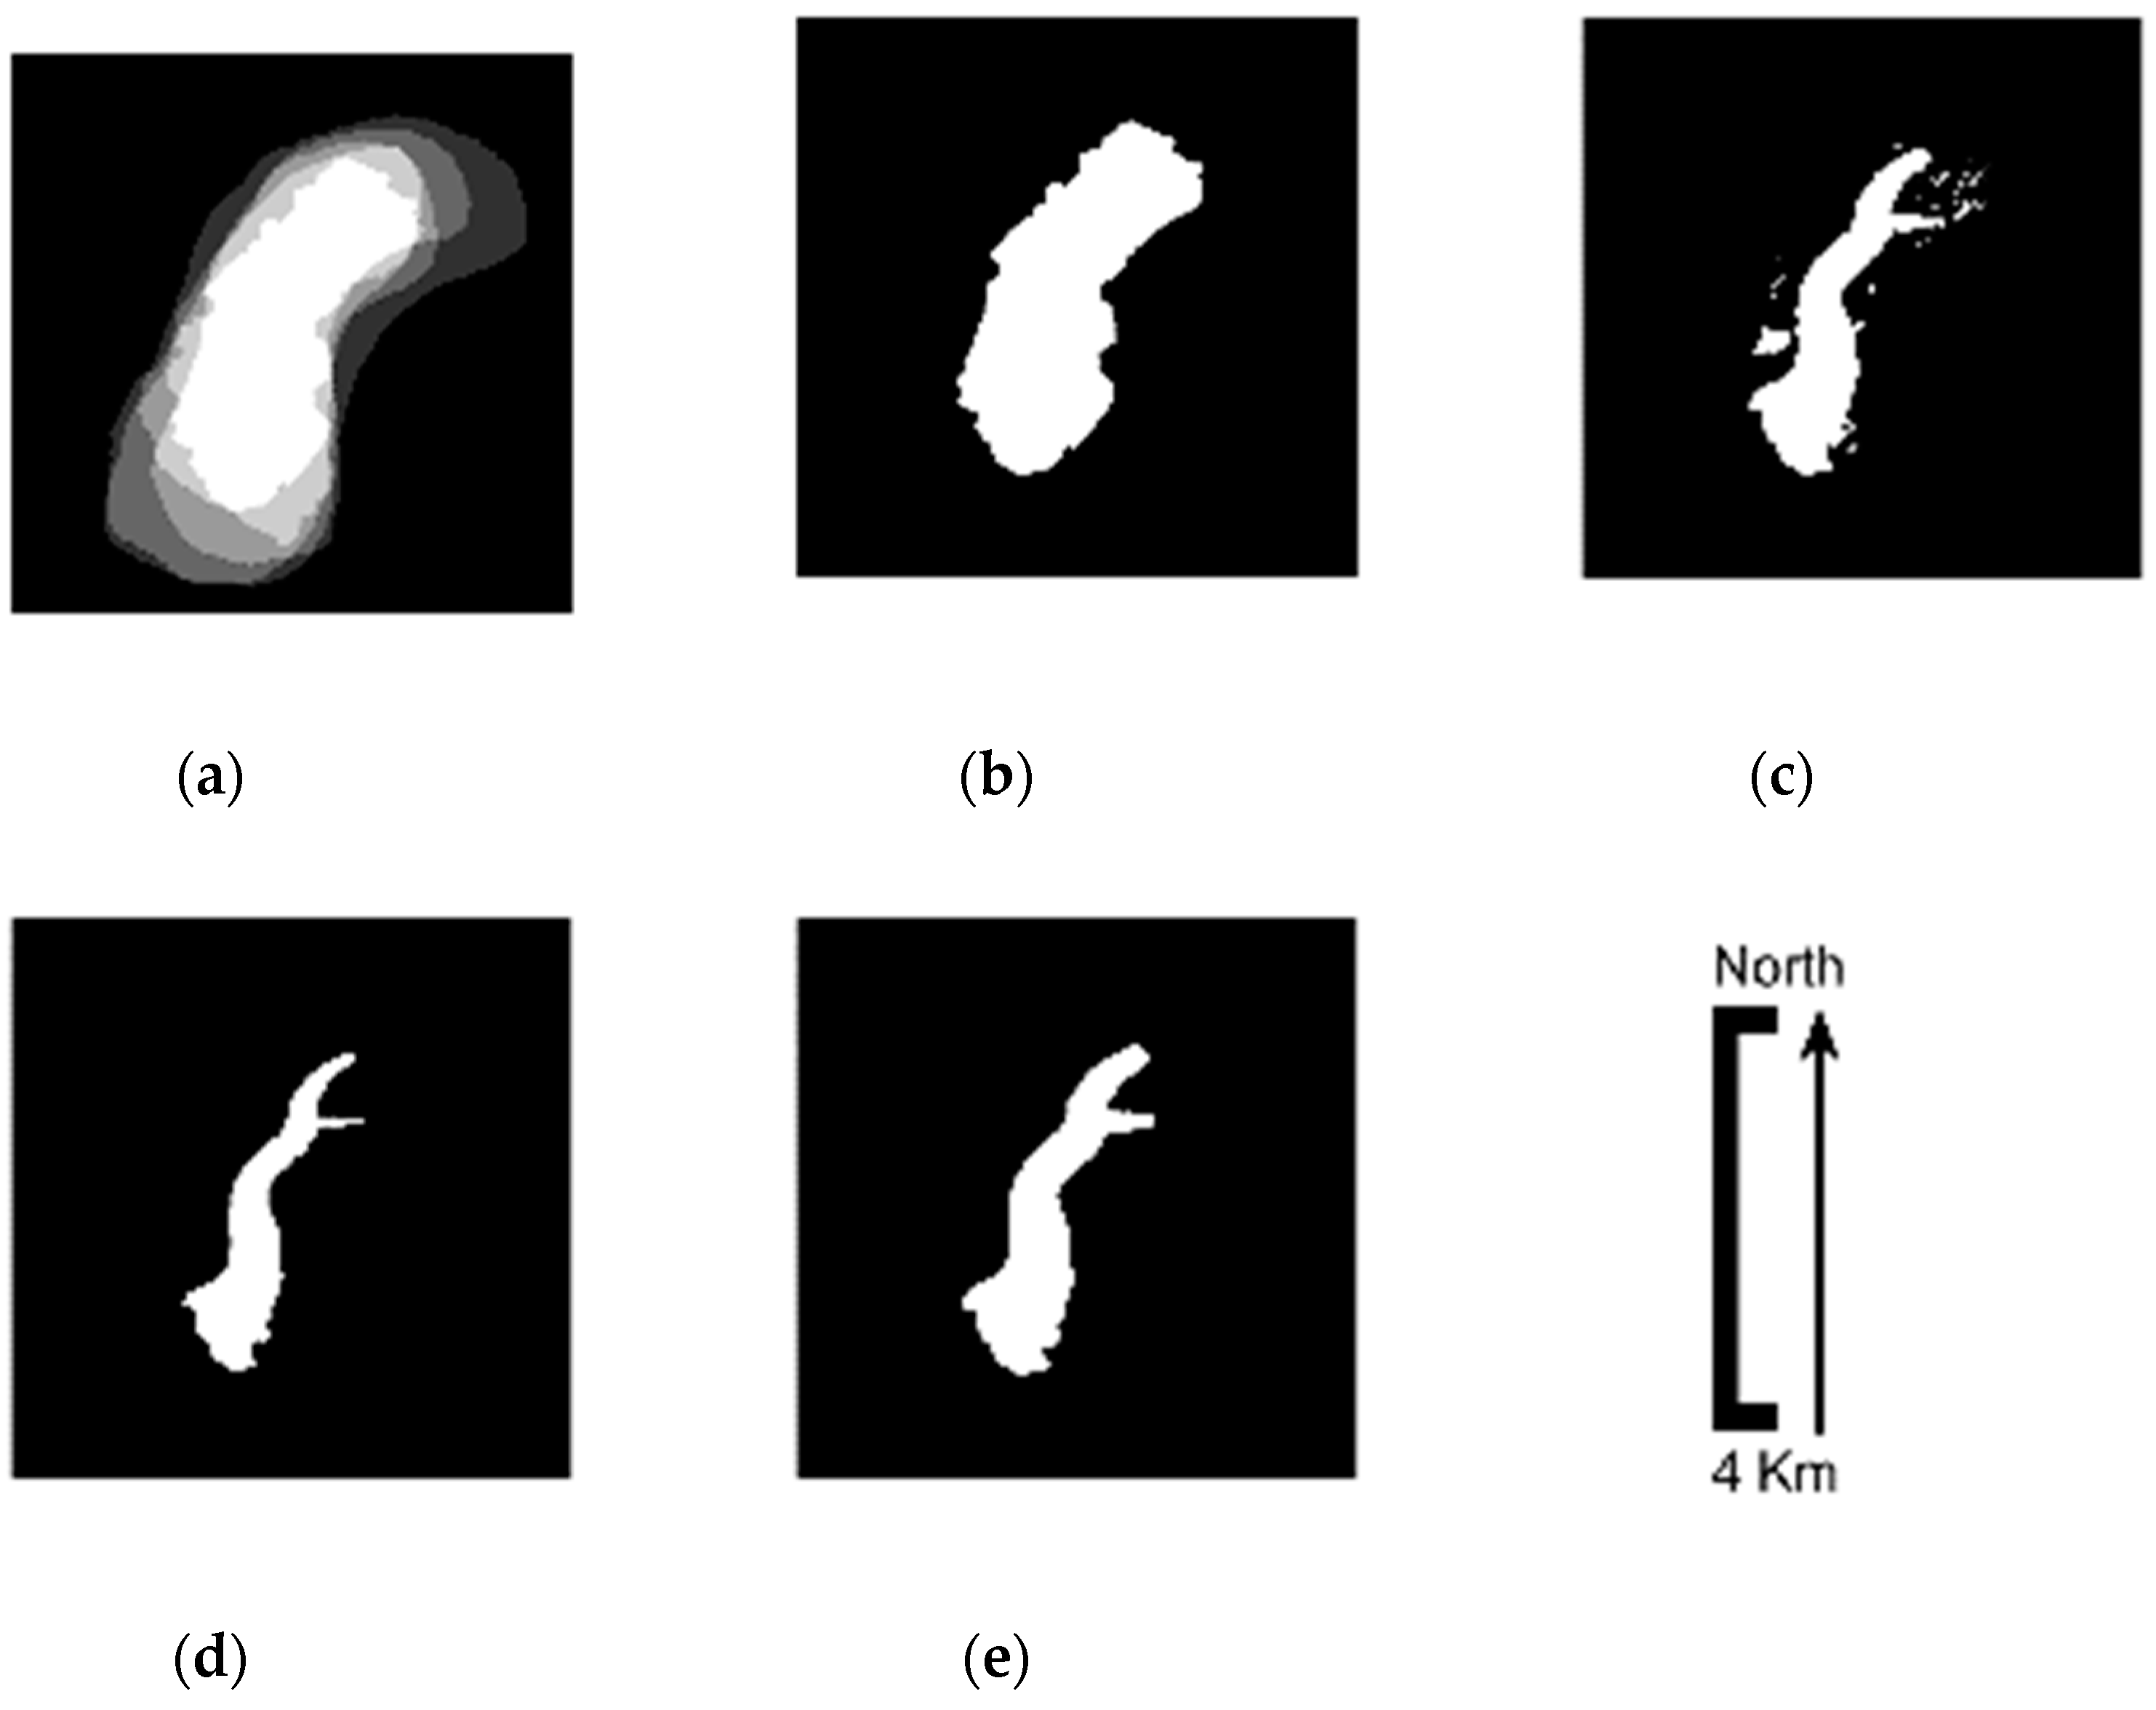
\includegraphics[width=0.9\textwidth]{glacier_masks.png}
    \caption{Steps for defining the final mask for defining the glacier boundaries: (a) binary mask defining the valid area of each survey overlapped; (b) common area between the masks; (c) high-variability area (i.e., areas for which the height difference between consecutive survey epochs was greater than 10 m); (d) filtered high-variability area; (e) buffered high-variability area, i.e., considered glacier shape. }
    \label{fig:2:glacier_masks}
\end{figure}

To compare DSM from different surveys, now at a consistent spatial resolution (0.5 m), a joint mask referring to the glacier body only and excluding surrounding areas was required.
To this end, the five binary masks defining the valid areas of each survey were superimposed, and only fully overlapped cells were considered (\figref{fig:2:glacier_masks}b).
A data-driven approach was pursued to identify the glacier body boundaries. 
In fact, low or even null altitude variability over time was expected in the surrounding areas, while cells referring to the glacier body were expected to show detectable changes in altitude. 
\figref{fig:2:glacier_masks}c shows the binary mask representing the cells for which the height difference between consecutive survey epochs was larger than 10 m. 
The shape of the glacier's body is recognizable. 
This mask was then refined by applying the same iterative procedure previously presented for the valid area identification, which first removed isolated areas and cleaned glacier borders (\figref{fig:2:glacier_masks}d) and then applied a buffer around it also to comprise lateral moraines expected to remain almost unchanged over time (\figref{fig:2:glacier_masks}e). 
The obtained final glacier mask (now covering about a surface of \SI{1.78}{\kilo\meter\squared}) was then applied to the interpolated DSMs.

\subsection{Glacier evolution analysis}\label{sec:2:glacier_evolution}

The final masked DSMs allowed spatial analyses of the glacier surface by comparing the measured altitude variations, quantifying volume variations, and evaluating the long-term morphology evolution from 1977 to 2019. 
First, the DSMs were analyzed in absolute terms, i.e., regarding their altitude variability range and the spatial distribution of areas classified based on their measured altitude. 

Additionally, relative comparisons were conducted to quantify the effects of accumulation and ablation processes on Belvedere Glacier over time.
Because the different DSMs were georeferenced and consistent in spatial resolution, volume variations could be computed by Dem of Difference (DoD).
Cumulate volume variations were obtained, taking the 1977 DSM as a reference, while average annual volume losses/gains were obtained in the considered periods.

\section{Results}\label{sec:2:results}

\subsection{SfM-MVS}\label{sec:2:res_reconstruction}

\begin{figure}[hb]
    \centering
    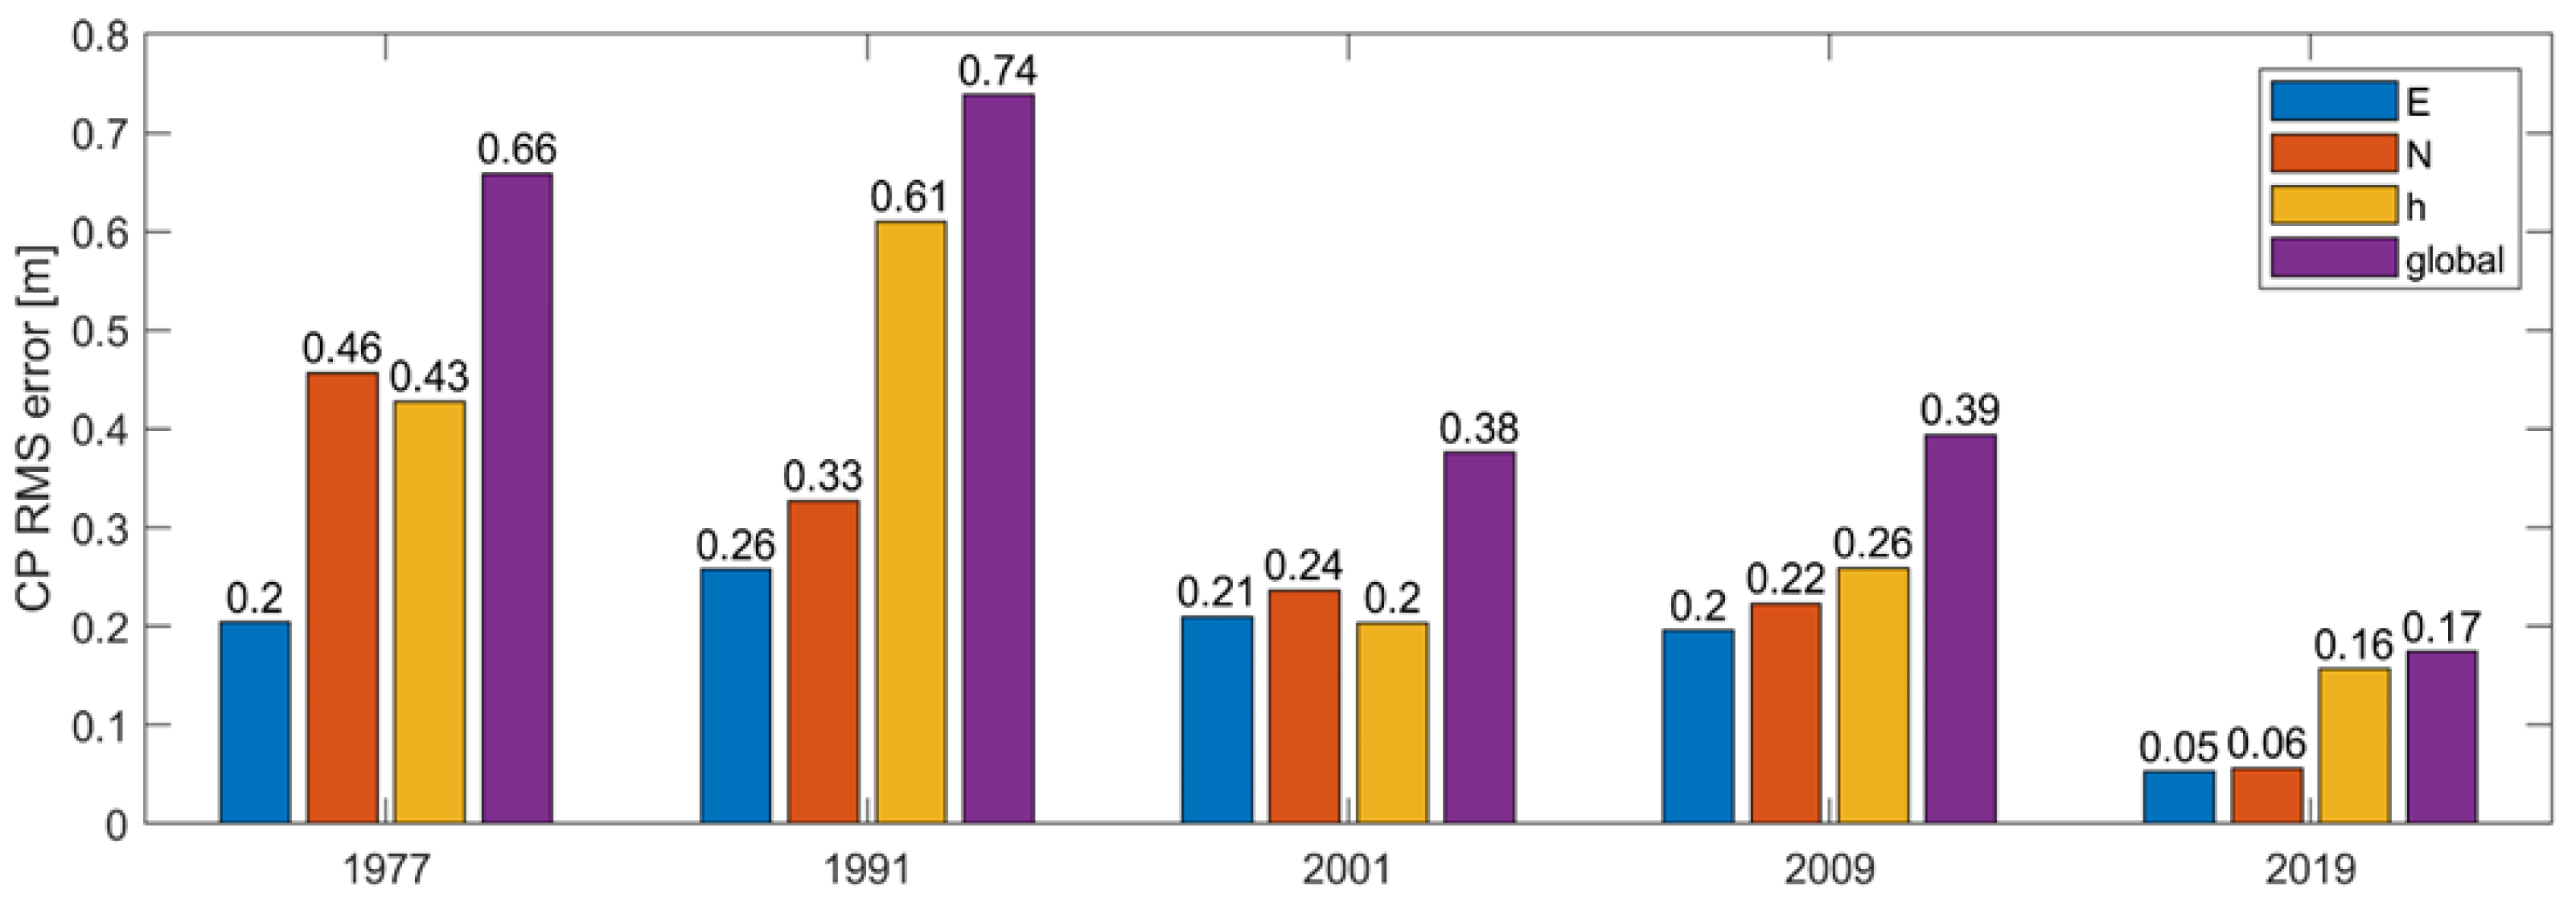
\includegraphics[width=1\textwidth]{cp_error.png}
    \caption{Model accuracy comparison in terms of RMS error on CPs. }
    \label{fig:2:cp_error}
\end{figure}

Eight CPs distributed mainly along the glacier moraines were used to assess the accuracy of the three historical models, while six CPs were used for the 2009 dataset \figref{fig:2:cp_error}.
The 1977 and 1991 models obtained global RMSEs of about 0.66 m and 0.74 m, respectively, while the 2001 and 2009 models obtained similar RMSEs of about 0.38 m.
In all cases, these values were comparable to the average GSD of the aerial images. Regarding the 2019 survey, the model accuracy was assessed by 10 CPs, resulting in an RMSE error of 0.17 m, comparable to three times the GSD. 
This was due to the low quality of the camera employed. 
Nevertheless, as the GSD was on the order of magnitude of the centimeter, the model accuracy was still higher than that of the older flights.

Starting from the solution obtained with the Agisoft Metashape SfM pipeline, an MVS approach was used to compute image depth maps, dense point clouds, orthophotos, and DSMs. 
The number of points in each PC and the density of each dense cloud are summarized in \tabref{tab:2:pcd_density}.
While the PC size was strictly related to the survey coverage, the PC average density was directly related to the GSD of the original photogrammetric survey, indicating the capability of resolving finer details.

\begin{table}
    \centering
    \caption{Point cloud (PC) numbers of points and volumetric densities.}
    \label{tab:2:pcd_density}
    \begin{tabular}{lccccc}
        \hline
        & 1977 & 1991 & 2001 & 2009 & 2019 \\
        \hline
        PC size [pts] & 8,962,182 & 4,296,638 & 12,504,582 & 17,595,703 & 112,293,439 \\
        PC average density [pts/m\textsuperscript{3}] & 1.56 & 1.08 & 1.58 & 2.67 & 26.40 \\
        \hline
    \end{tabular}
\end{table}

Orthophotos and DSMs were computed with a GSD of \SI{0.50}{\meter} for the historical datasets of 1977, 1991, and 2001, \SI{0.40}{\meter} for the digital aerial dataset of 2009, and \SI{0.20}{\meter} for the UAV dataset of 2019.
The computed orthophotos are visible in Appendix \ref{app:orthophotos}.

\subsection{Point cloud pre-processing}\label{sec:2:res_preproc}

Based on the preliminary processing described in \secref{sec:2:pcd_preproc}, reliable estimates of surveyed surface coverage and average density of the original point clouds were quantified (\tabref{tab:2:pcd_surface_coverage}).
Surface coverage was obtained by multiplying the number of nonzero values of the binary masks of the valid area of each survey and the DSM cell size (\SI{0.25}{\square\meter}). 
The ratio between the number of nonempty cells in the original and interpolated DSMs indicated the average data density of the point clouds in the considered surveyed areas. 

\begin{table}[ht]
  \centering
  \caption{Summary of Surface Coverage and Average Density of Point Clouds}
  \label{tab:2:pcd_surface_coverage}
  \begin{tabular}{lccccc}
    \hline
    & 1977 & 1991 & 2001 & 2009 & 2019 \\
    \hline
    Surface Coverage [\%] & 5.53 & 9.41 & 7.17 & 5.98 & 4.33 \\
    Data Density [cells/m\textsuperscript{2}] & 37\% & 11\% & 39\% & 60\% & 94\% \\
    \hline
  \end{tabular}
\end{table}

The numbers in \tabref{tab:2:pcd_surface_coverage} allow evaluating the impact of the chosen grid spacing when gridding the point clouds. 
With 0.5 m grid spacing, the 2019 survey (the most detailed one) required a few empty cells to be interpolated, about 6\%, thus closely fully exploiting its high spatial resolution. 
A finer grid would require increasing the number of interpolated cells (thus increasing the required memory allocation for matrix manipulation) without adding information, particularly for the historical surveys.
On the other hand, a coarser resolution would require downsampling the surveyed detailed DSM, potentially losing finer details. 
With the chosen grid spacing, the minimum amount of interpolation was needed, while the full potential of more recent and detailed surveys was preserved. 
Furthermore, the surface coverage of the different surveys was quite different, introducing the second aspect to be addressed to complete the required preprocessing of the point clouds.

\begin{table}[ht]
  \centering
  \caption{Minimum and Maximum Altitudes (a.s.l.) of the Glacier at Different Epochs}
  \label{tab:2:glacier_altitudes}
  \begin{tabular}{lccccc}
    \hline
    Epoch & 1977 & 1991 & 2001 & 2009 & 2019 \\
    \hline
    Min Altitude (m) & 1820.72 & 1823.60 & 1824.44 & 1826.23 & 1825.64 \\
    Max Altitude (m) & 2381.11 & 2385.07 & 2350.37 & 2339.43 & 2349.36 \\
    \hline
  \end{tabular}
\end{table}

\subsection{Glacier evolution analysis}\label{sec:2:res_glacier_evolution}

\begin{figure}[ht]
    \centering
    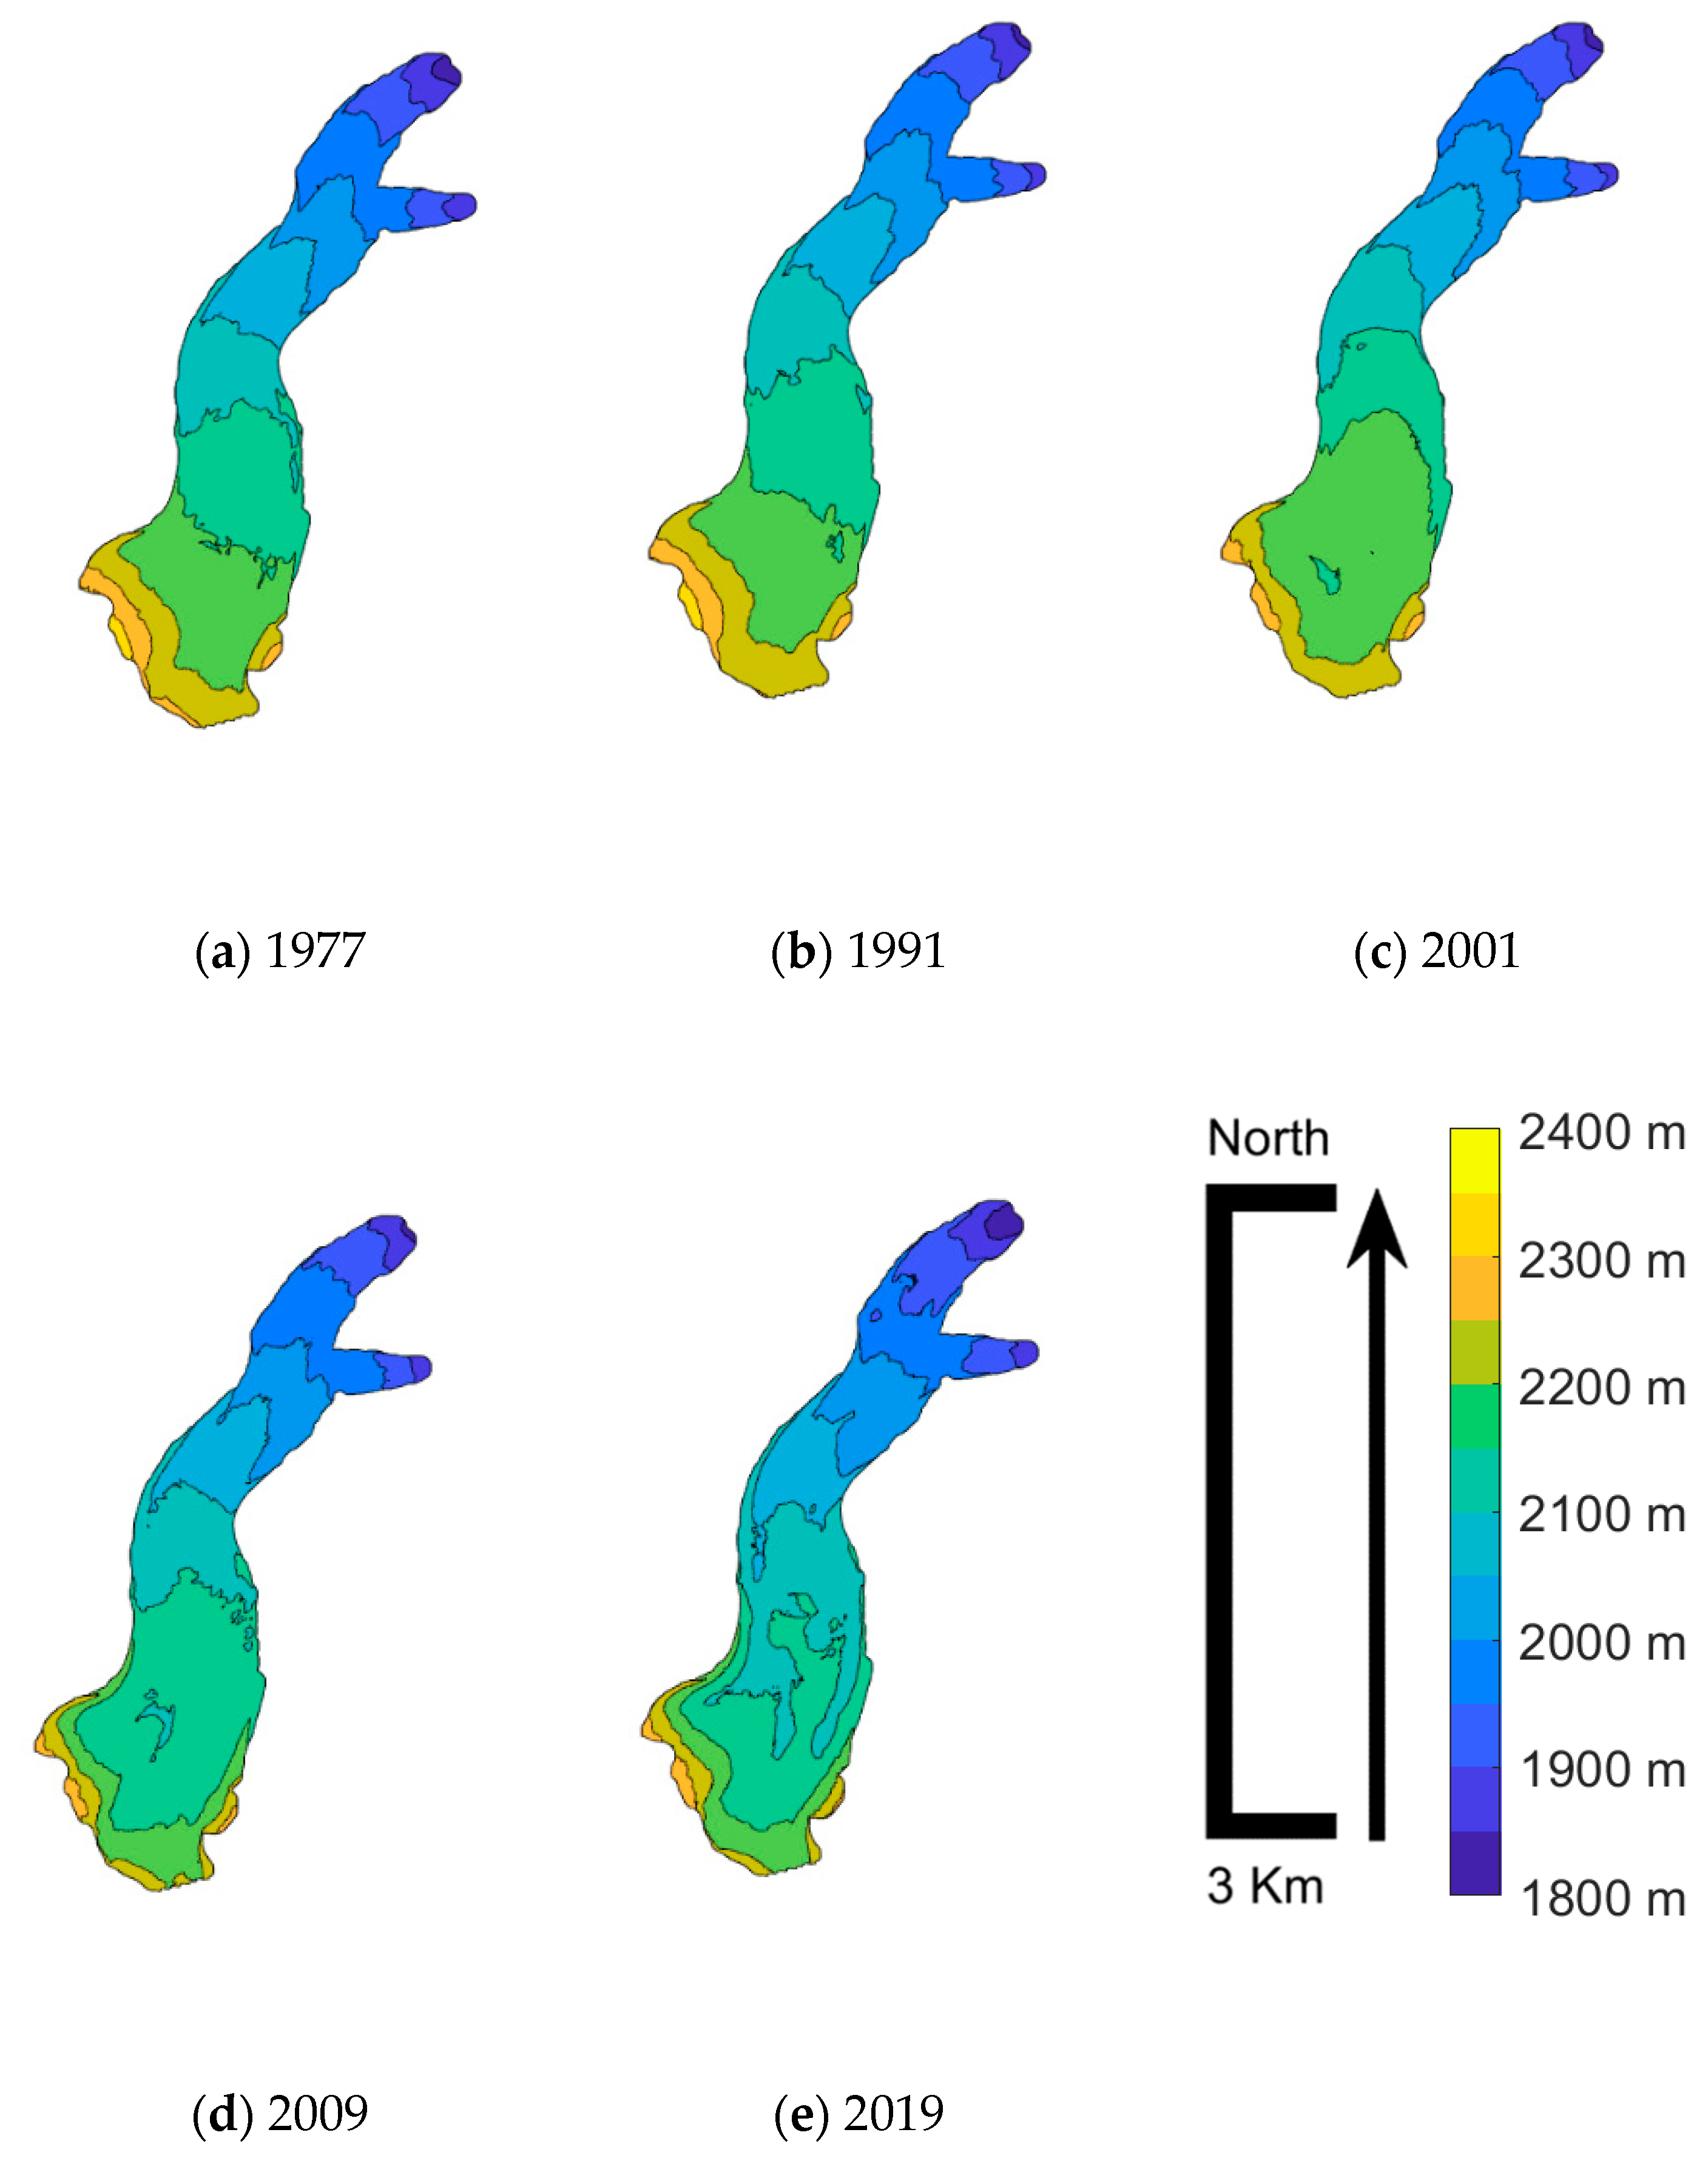
\includegraphics[height=0.9\textheight]{results_contours.png}
    \caption{Glacier contours at different epochs: (a) 1977; (b) 1991; (c) 2001; (d) 2009; (e) 2019.}
    \label{fig:2:results_contour}
\end{figure}

The minimum and maximum altitudes of the glacier extracted from each DSM are shown in \tabref{tab:2:glacier_altitudes}.
The minimum values ranged between 1820 m and 1826 m, while maximum values ranged between 2339 m and 2385 m. 
The stability of the minimum values can be justified by the area masking. 
Minimum altitudes likely occurred near the glacier terminus, and the mask buffering could have comprised points surveyed at the terminal lobes.
On the other hand, the variability of the maximum glacier heights likely occurred closer to mountainous peaks along the surveyed glacier accumulation area, located in the SW region of the mask, where mass balance can benefit from events such as avalanches or particular meteorological conditions immediately before the epoch of the surveys.

\figref{fig:2:results_contour} presents glacier contour altitudes between 1800 and 2400 m, to comprise the maximum altitude range measured by the five surveys with a contour interval of 50m.
Compared to the 1977 DSM (\figref{fig:2:results_contour}a), 1991 DSM cells classified in the range 2200–2400 m remained almost unchanged while the following contour lines gradually moved toward a valley, clearly indicating a mass accumulation (\figref{fig:2:results_contour}b).
The following 2001 survey showed a continuation in these areas of the trend of increasing altitude toward the glacier terminus. 
Still, an altitude decrease was observed in the SW cells of the accumulation area (note the extension of the altitude class 2200–2250 m in \figref{fig:2:results_contour}c), and cells of the highest altitude class were practically absent (see \tabref{tab:2:glacier_altitudes}). 
The 2009 DSM showed different behavior (\figref{fig:2:results_contour}d). 
Lower contour lines retreated toward peaks, approximately in the same location as in 1977, while the 2150–2200 m range greatly retreated and covered a large part of the glacier toward the accumulation area.
The most recent 2019 DSM (\figref{fig:2:results_contour}e) again showed a general retreat trend of lower contour lines, with no sharp transition in the range of 2100–2200 m (probably due to high surface ablation phenomena) and no great variation in the remaining areas in the range of 2200–2350 m.

\begin{table}[ht]
  \centering
  \caption{Glacier Volume Gain/Loss in the Four Considered Periods}
  \label{tab:2:glacier_volume_variations}
  \begin{tabular}{lcccc}
    \hline
    Period & 1977--1991 & 1991--2001 & 2001--2009 & 2009--2019 \\
    \hline
    $\Delta$Vol (millions m\textsuperscript{3}) & +10.06 & +10.61 & $-$47.78 & $-$27.16 \\
    Yearly $\Delta$Vol (millions m\textsuperscript{3}/year) & +0.72 & +1.06 & $-$5.97 & $-$2.72 \\
    Cumulated $\Delta$Vol (millions m\textsuperscript{3}) & +10.06 & +20.66 & $-$27.12 & $-$54.28 \\
    \hline
  \end{tabular}
\end{table}

Volume variations obtained by DoD are shown in \tabref{tab:2:glacier_volume_variations}.
Cumulated volume variations are computed considering the 1977 DSM as a reference.
The numbers in \tabref{tab:2:glacier_volume_variations} confirm what was found by analyzing the glacier contour variations but from a different perspective. 

Between 1977 and 2001, the glacier's volume increased substantially by \SI[retain-explicit-plus]{+20.66e6}{\cubic\meter}.
Notably, the rate of expansion accelerated during the period 1991-2001.
During this period, the glacier gained volume 50\% faster than the previous decade, increasing from \SI[retain-explicit-plus]{+0.72e6}{\cubic\meter\per\year} to \SI[retain-explicit-plus]{+1.06e6}{\cubic\meter\per\year}.
The glacier expansion continued until the surge event of 2000-2002 \citep{Haeberli2002, Kaab2004, Mortara2009}.

Since 2001, the glacier has undergone severe retreat, losing a total of \SI{-74.94e6}{\cubic\meter} of ice volume between 2001 and 2019.
From 2001 to 2009, the average yearly volume decrease was \SI{-5.97e6}{\cubic\meter\per\year}, reducing the volume by \SI{-27.12e6}{\cubic\meter} relative to the initial 1977 measurement, despite prior accumulation.

While the negative trend persisted from 2009 to 2019, the rate of loss slowed (\SI{-2.72e6}{\cubic\meter\per\year}).
Over the 42-year observation period (1977-2019), the glacier experienced a net loss of \SI{-54.28e6}{\cubic\meter}.

\begin{figure}
    \centering
    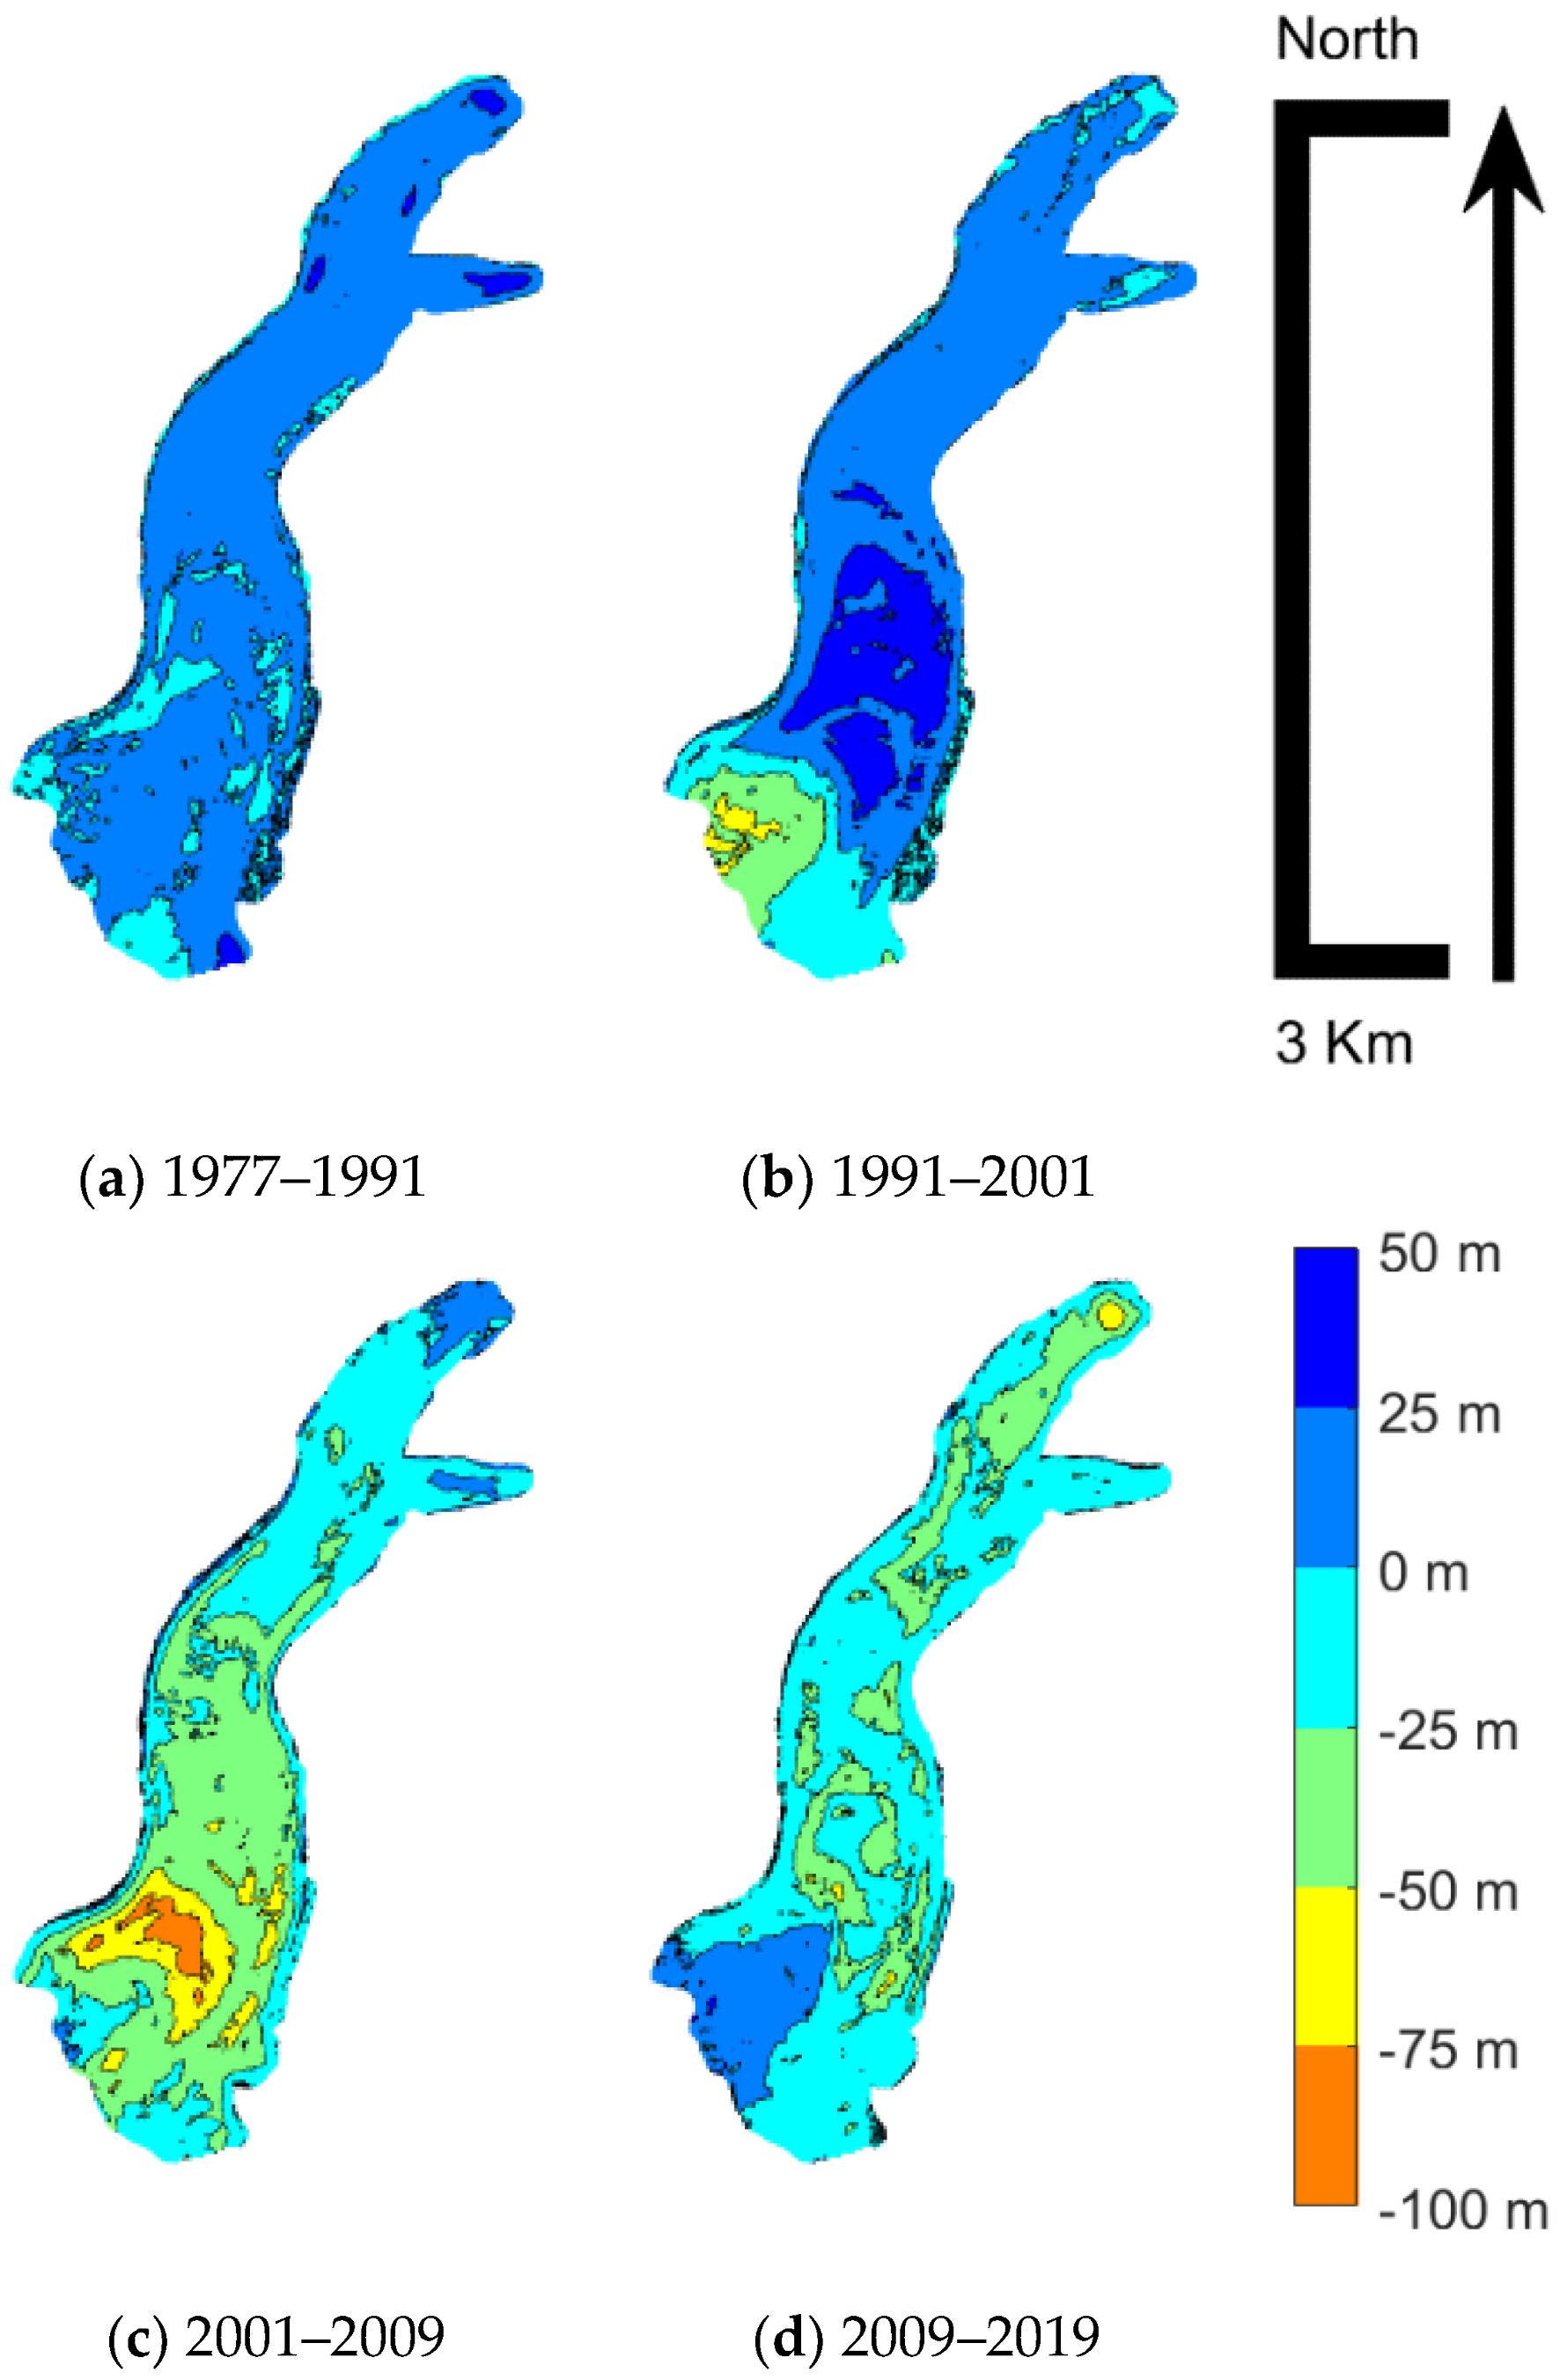
\includegraphics[width=0.9\textwidth]{results_volumes_variations.png}
    \caption{Binned glacier altitude variations in different periods with bin size set to 25 m: (a) 1977–1991; (b) 1991–2001; (c) 2001–2009; (d) 2009–2019. }
    \label{fig:2:volume_variations}
\end{figure}

The reported volume gains or losses refer to the whole glacier surface, but it could be interesting to investigate local variations. 
\figref{fig:2:volume_variations} classifies glacier areas in terms of altitude variation, with contour intervals of 25 m. 
The volume increase was quite distributed in the first considered period, from 1977 to 1991. 
Glacier terminus advancement was visible, and volume decrease was measured in small portions at higher altitudes. 
The following period, 1991–2001, saw an important volume accumulation in the central part of the glacier, which was partially counterbalanced at higher altitudes. 
The following periods showed general volume loss, which was particularly important in the higher portion between 2001 and 2009 and was distributed until the terminus (see the northern one) in the period 2009–2019.

\subsection{Comparison with previous studies}

Several studies focused on understanding and quantifying Belvedere Glacier dynamics. 
\citet{Diolaiuti2003} digitalized two large-scale topographic maps to interpolate DSMs and estimate volume variations between 1957 and 1991. 
They found a positive volume difference of \SI{+22.7e6}{\cubic\meter}, which translates to an average rate of \SI{\sim0.69e6}{\cubic\meter\per\year} (assuming a linear volume variation between 1957 and 1991). 
This aligns with the yearly volume variation rate estimated in this study between 1977 and 1997, equal to \SI{+0.72e6}{\cubic\meter\per\year}.
The results obtained by \citet{Diolaiuti2003} agrees with those obtained by \citet{Roethlisberger1985}, who estimated an increase of the glacier height of 
\SI{+1.5}{\meter\per\year} between 1983 and 1985.

% References
\makechapterbibliography{}